\documentclass[11pt]{article}
\usepackage[T1]{fontenc}
\usepackage{lmodern,microtype}
\usepackage[margin=1in]{geometry}
\usepackage{amsmath,amssymb,amsthm,mathtools}
\usepackage{enumitem}
\usepackage{needspace,placeins}
\usepackage{tikz}
\usetikzlibrary{arrows.meta,positioning,calc,patterns}
\usepackage[colorlinks=true,linkcolor=blue!45!black,citecolor=blue!45!black,urlcolor=blue!45!black]{hyperref}
\newtheorem{theorem}{Theorem}[section]
\newtheorem{lemma}[theorem]{Lemma}
\newtheorem{proposition}[theorem]{Proposition}
\newtheorem{corollary}[theorem]{Corollary}
\theoremstyle{definition}
\newtheorem{definition}[theorem]{Definition}
\theoremstyle{remark}
\newtheorem{remark}[theorem]{Remark}
\numberwithin{equation}{section}
\newcommand{\C}{\mathbb C}
\newcommand{\R}{\mathbb R}
\newcommand{\N}{\mathbb N}
\newcommand{\Z}{\mathbb Z}
\newcommand{\E}{\mathbb E}
\newcommand{\one}{\mathbf 1}
\newcommand{\norm}[1]{\left\lVert#1\right\rVert}
\newcommand{\abs}[1]{\left|#1\right|}
\newcommand{\ip}[2]{\left\langle#1,#2\right\rangle}
\DeclareMathOperator{\diag}{diag}
\DeclareMathOperator{\supp}{supp}
\DeclareMathOperator{\Ad}{Ad}
\DeclareMathOperator{\Tr}{Tr}
\DeclareMathOperator{\tr}{tr}
\DeclareMathOperator{\dist}{dist}
\DeclareMathOperator{\rank}{rank}
\DeclareMathOperator{\clip}{clip}
\title{Approximation Paving over Arbitrary Maximal Abelian Subalgebras}
\author{OpenAI}
\date{September 25, 2026}
\hypersetup{pdftitle={Approximation Paving over Arbitrary Maximal Abelian Subalgebras},pdfauthor={OpenAI}}
\begin{document}
\maketitle
\begin{abstract}
We prove the approximation-paving conjecture of Popa and Vaes for every
maximal abelian subalgebra of a complex von Neumann algebra. For each
\(0<\varepsilon<1\), every self-adjoint operator is a strong limit of
self-adjoint operators of norm at most three times its norm, each admitting a
norm paving with error at most \(\varepsilon\) times the approximant's own
norm. The number of projections is at most \(C\varepsilon^{-6}\) for a
universal constant \(C\). No separability or conditional-expectation
hypothesis is required.
\end{abstract}
\section{Introduction}\label{sec:introduction}

Let \(A\) be a maximal abelian unital \(*\)-subalgebra, or MASA, of a
complex von Neumann algebra \(M\).
For a finite partition \(\mathcal P=(p_i)_{i=1}^r\) of the unit by
projections in \(A\), write
\[
 C_{\mathcal P}(z)=\sum_{i=1}^r p_i z p_i .
\]
Norm paving asks whether \(C_{\mathcal P}(z)\) can be made close in
operator norm to an element of \(A\). Approximation paving allows a
bounded perturbation of \(z\) within any prescribed strong-operator
neighborhood before choosing the partition.

Kadison and Singer posed the pure-state extension problem for the atomic
diagonal MASA of \(\mathcal B(\ell^2)\) \cite{KS59}. Anderson formulated its
diagonal paving counterpart \cite{Anderson79}, and Marcus, Spielman and
Srivastava resolved it by mixed characteristic polynomials \cite{MSS15}.
For general MASAs, ordinary norm paving of the original operator is too
restrictive: in the separable-predual setting, it characterizes type I
algebras with a normal expectation onto the MASA
\cite[Theorem~3.3]{PV15}. Popa and Vaes introduced strong-operator and
approximation versions of paving and conjectured that every MASA has
both properties \cite[Definitions~2.2--2.3 and Conjecture~2.8(1)]{PV15}.
We resolve the approximation-paving assertion of that conjecture positively.

Popa proved norm paving in ultraproducts of singular finite MASAs,
and hence strong-operator paving in the original finite inclusions
\cite{Popa14}. Popa and Vaes established strong-operator and approximation
paving for type I algebras with separable predual and for Cartan
inclusions in amenable algebras or arising from free ergodic profinite
actions \cite[Sections~3--4]{PV15}. For singular finite MASAs they
obtained quadratic paving bounds \cite[Theorem~5.1]{PV15}, later
sharpened in \cite{PV16}. These restricted cases do not provide the
expectation-free approximation theorem below.

\Needspace{16\baselineskip}
\begin{theorem}\label{thm:main}
There is a universal constant \(C_{\mathrm{ap}}>0\) such that for every
\(0<\varepsilon<1\) there is an integer
\(R(\varepsilon)\leq C_{\mathrm{ap}}\varepsilon^{-6}\)
with the following property.
Let \(M\subseteq\mathcal B(H)\) be a complex von Neumann algebra,
let \(A\subseteq M\) be a MASA, and let \(x=x^*\in M\).
For every finite \(F\subset H\) and every \(\delta>0\), there exist
\(y=y^*\in M\), a partition \(\mathcal P=(p_i)_{i=1}^{R(\varepsilon)}\)
of the unit in \(A\), and \(a=a^*\in A\), such that
\[
 \norm{y}\leq3\norm{x},\qquad
 \norm{(y-x)\xi}<\delta\quad(\xi\in F),
\]
and
\[
 \norm{a}\leq\norm{y},\qquad
 \norm{C_{\mathcal P}(y)-a}\leq\varepsilon\norm{y}.
\]
Zero projections may be included in the partition.
\end{theorem}

Thus the norm-control constant is universal, and the number of
projections is independent of the algebra, its representation, the
operator, and the strong neighborhood. We do not optimize the
sixth-power bound.
The relative error in the theorem is measured against the actual
approximant's norm; a norming test vector and a final clipping argument
will ensure that normalization.

There is also a direct consequence for strong-operator paving when a
normal expectation exists. In its definition, the compression is
estimated on a large projection whose complement lies in a prescribed
strong neighborhood of zero.

\begin{corollary}\label{cor:so-paving}
Suppose that a MASA \(A\subseteq M\) is the range of a normal
conditional expectation. For each \(0<\varepsilon<1\) there is an
integer \(R_s(\varepsilon)\), independent of the inclusion, such that
for every \(x=x^*\in M\) and every strong-operator neighborhood
\(\mathcal V\) of zero, there exist an \(R_s(\varepsilon)\)-partition
\(\mathcal P\) in \(A\), an \(a=a^*\in A\) with
\(\norm{a}\leq\norm{x}\), and a projection \(q\in M\) with
\(\one-q\in\mathcal V\), satisfying
\[
 \norm{q(C_{\mathcal P}(x)-a)q}\leq\varepsilon\norm{x}.
\]
\end{corollary}
The proof is given in Section~\ref{gen:consequences}.

The separate companion \cite[Theorem~1.1]{OAQuadratic26} proves a direct
quadratic strong-operator paving bound for the original operator.
Theorem~\ref{thm:main} instead norm-paves a nearby bounded operator,
with error relative to that approximant's norm. The two main proofs are
independent; the conversion in Corollary~\ref{cor:so-paving} retains its normal-expectation
hypothesis. We claim no quadratic bound for \(R(\varepsilon)\).

\begin{corollary}[Quadratic approximation paving for expected MASAs]
\label{cor:quadratic-expected-approximation}
There is a universal constant \(C>0\) such that for every
\(0<\varepsilon<1\) one can choose an integer
\(N(\varepsilon)\leq C\varepsilon^{-2}\) with the following property.
If the MASA \(A\subseteq M\) is the range of a normal conditional expectation,
then the conclusion of Theorem~\ref{thm:main} holds with
\(N(\varepsilon)\) in place of \(R(\varepsilon)\).
\end{corollary}
The proof is given in Section~\ref{gen:consequences}.

\paragraph{The measured argument.}
The first part of the proof develops a measurable version of
one-sided matrix paving for nonsingular equivalence relations.
The finite paving-polynomial framework of
\cite{RL20,RS21} supplies the starting point. Its stable expected
determinants yield local spectral probabilities and spectral-shift
functions.
A buffered pinning lemma selects a color while increasing the
diagonal penalty by a fixed universal factor and controlling the
increase of positive-root mass.
The initial root estimate from \cite[Lemma~24 and proof of Theorem~25]{RS21}
is derived here from \cite[Theorems~4.1 and~5.1]{MSS15}, using
positive-defect completion and deletion of added Gram columns.

Nonsingularity is handled by passing to the Maharam extension, where
mass transport is invariant, and weighting the matrix by the height
variable. Uniform comparisons between slabs allow the pinning
decisions to descend to a single coloring of the base.
Sparse random updates then control the accumulated cost.
Only local independence is needed; auxiliary graph colorings do not
increase the number of colors in the final paving.
The slab comparison and buffered-pinning estimates isolate the two
uniformity issues in this passage from finite matrices to measurable
operators.

\paragraph{The operator-algebra argument.}
For a MASA in the centralizer of a faithful normal state, we first pave
the algebra generated by its normalizers, using the
Feldman--Moore representation \cite{FM77} and the measured theorem.
The complementary part has diffuse left--right kernels.
We adapt the free-product matrix dilation of
\cite[proof of Theorem~5.1]{PV15}, using random diagonal phases to
obtain asymptotic freeness with respect to the induced state.
The proof controls the moments and their concentration without assuming
traciality, using analytic right multiplication for the modular group.

Finally, a separable reduction preserves the partition bounds.
The corner carrying centralizing normal positive functionals has a
normal expectation; on the complementary corner, almost disjoint
conjugate states produce positive contractions with small diagonal
compressions. A three-corner construction preserves the original
off-diagonal entries until the final partition is chosen.
This is the step that removes the normal-expectation hypothesis.

All new estimates needed for these passages are proved below.
We use established structure theorems for conditional expectations,
standard form, type I algebras and free products, with their hypotheses
specified at the points of application.

Section~\ref{sec:preliminaries} fixes the state-topology tools;
Sections~\ref{poly:section}--\ref{sec:pinning} prove the measured paving
theorem, Section~\ref{sec:expected} handles the state-preserving case,
and Section~\ref{gen:section} removes the remaining hypotheses.

\clearpage
\tableofcontents
\clearpage
\section{State topology and bounded sequence quotients}
\label{sec:preliminaries}

All algebras and Hilbert spaces are over \(\C\).
A MASA is automatically a von Neumann algebra: its relative commutant
equals itself, by taking real and imaginary parts.
Partitions are finite indexed families of orthogonal projections with
sum \(\one\); we allow zero projections.
For a self-adjoint operator \(t\), let \(t_+\) denote its positive part.
We use the same functional-calculus notation for continuous real
functions, including
\[
 \clip_c(t)=\max(-c,\min(t,c)),\qquad c>0.
\]

Suppose for this section that \(M\) has a faithful normal state
\(\varphi\), and \(A\subseteq M_\varphi\) is a MASA in its centralizer.
Here
\[
 M_\varphi=\{a\in M:\varphi(az)=\varphi(za)\text{ for all }z\in M\}.
\]
The modular group fixes \(A\) pointwise. The conditional-expectation
theorem gives a faithful normal \(\varphi\)-preserving expectation
\(E_A:M\to A\); see \cite{Takesaki72} or \cite[Theorem~6.6]{Hiai20}.
Set
\[
 \norm{z}_\varphi=\varphi(z^*z)^{1/2},
 \qquad
 \norm{z}_\varphi^\#=\norm{z}_\varphi+\norm{z^*}_\varphi.
\]
On bounded sets these seminorms determine, respectively, the
\(\sigma\)-strong and \(\sigma\)-strong* topologies.
Indeed, in the faithful state representation,
\(\norm{z}_\varphi=\norm{z\xi_\varphi}\), and \(M'\xi_\varphi\) is
dense. Boundedness therefore promotes convergence on \(\xi_\varphi\)
to strong convergence on all vectors. The bounded
\(\sigma\)-strong topology is intrinsic to the von Neumann algebra.
Apply the same reasoning to adjoints for the second assertion.
In standard \(L^2(M)\) notation we write
\(\xi_\varphi=\varphi^{1/2}\). Elements of \(A\) commute with this
vector under the left and right actions.

\begin{lemma}\label{lem:compression-net}
Every \(A\)-partition compression \(C_{\mathcal Q}\) preserves
\(\varphi\) and is contractive for both state seminorms.
As \(\mathcal Q\) refines through all finite \(A\)-partitions,
\[
 C_{\mathcal Q}(z)\longrightarrow E_A(z)
 \quad\text{in }\norm{\cdot}_\varphi^\#
 \qquad(z\in M).
\]
The same holds along any refining sequence of partitions generating \(A\).
\end{lemma}
\begin{proof}
The centralizer identity gives
\(\varphi(C_{\mathcal Q}(z))=\varphi(z)\).
Compression is unital completely positive, so its Schwarz inequality
gives state-norm contraction; apply it to adjoints as well.
On the state Hilbert space the compression is implemented by the
orthogonal projection
\[
 \zeta\longmapsto\sum_{q\in\mathcal Q}q\zeta q.
\]
These projections decrease under refinement. Their action on
\(z\varphi^{1/2}\) is
\(C_{\mathcal Q}(z)\varphi^{1/2}\).
Meanwhile the operators \(C_{\mathcal Q}(z)\) are uniformly bounded.
Every ultraweak cluster point commutes with all projections of \(A\),
and hence is in \(A\). Since
\(E_A C_{\mathcal Q}(z)=E_A(z)\), the cluster point equals \(E_A(z)\).
The Hilbert-space limit of the decreasing projections must therefore
be \(E_A(z)\varphi^{1/2}\).
Repeating for \(z^*\) proves the claim.
For a generating refining sequence, commuting with all of its
partition projections is already equivalent to commuting with \(A\),
so the same proof applies.
\end{proof}

The following quotient allows us to record vanishing state errors
while retaining norm estimates. Its multiplier condition matters
when \(\varphi\) is not tracial.

\Needspace{12\baselineskip}
\begin{lemma}\label{lem:sequence-quotient}
Let
\[
 \mathcal I_\varphi=
 \{(z_j)\in\ell^\infty(M):\norm{z_j}_\varphi^\#\to0\},
\]
and let
\[
 \mathcal C_\varphi=
 \{t\in\ell^\infty(M):
 t\mathcal I_\varphi\subseteq\mathcal I_\varphi,\
 \mathcal I_\varphi t\subseteq\mathcal I_\varphi\}.
\]
Then \(\mathcal C_\varphi\) is a unital \(C^*\)-algebra and
\(\mathcal I_\varphi\) is a closed two-sided ideal in it.
Constant sequences from \(M\) and all sequences in
\(\ell^\infty(A)\) belong to \(\mathcal C_\varphi\).
\end{lemma}
\begin{proof}
The set \(\mathcal I_\varphi\) is self-adjoint and norm closed.
If \(s,t\in\mathcal I_\varphi\), then
\[
 \norm{s_jt_j}_\varphi\leq
 \norm{s_j}\norm{t_j}_\varphi,\qquad
 \norm{(s_jt_j)^*}_\varphi\leq
 \norm{t_j}\norm{s_j^*}_\varphi ,
\]
so \(st\in\mathcal I_\varphi\).
The two multiplier conditions now show directly that
\(\mathcal C_\varphi\) is a unital, norm-closed \(*\)-algebra,
contains \(\mathcal I_\varphi\), and makes it an ideal.
Multiplication by a fixed bounded operator is continuous on bounded
sets for strong* convergence, so constant sequences are multipliers.

If \(a\in A\), then left multiplication has state-norm bound
\(\norm{a}\), and the centralizer property gives
\[
 \norm{ta}_\varphi^2
 =\varphi(a^*t^*ta)
 =\varphi(t^*t aa^*)
 \leq \norm{a}^2\varphi(t^*t).
\]
The last inequality follows from positivity, since
\(\varphi(t^*t b)=\varphi(b^{1/2}t^*t b^{1/2})\geq0\) for
\(b\geq0\) in \(A\).
The same estimates apply to adjoints, uniformly on bounded
\(A\)-sequences. Thus these sequences are multipliers.
\end{proof}

Write \([t_j]\) for an image in
\(\mathcal C_\varphi/\mathcal I_\varphi\).
A sequence of \(A\)-partitions of uniformly bounded size acts by
compression in this quotient.
If \(q\) refines \(p\), its compression applied to a \(p\)-compression
is its compression of the original element.
Since these maps are unital and positive, a common refinement
preserves separate scalar upper and lower bounds for a self-adjoint
element. In particular it preserves a norm bound.

We will also use the following direct consequence of functional calculus.
If a self-adjoint multiplier sequence \(T_j\) has
\(\norm{[T_j]}\leq c\), then
\[
 w_j=T_j-\clip_c(T_j)\in\mathcal I_\varphi,\qquad
 \norm{T_j-w_j}\leq c.
\]
If \(T_j\) is block diagonal for a partition, so is \(w_j\).
This converts the quotient estimates below into explicit corrections.

\section{Finite mixed polynomials and buffered pinning}\label{poly:section}

We develop a rule for fixing one vertex's color while controlling the
total positive-root mass of an expected characteristic polynomial.
The rule will be applied repeatedly in the measured paving argument;
its constants must therefore be independent of the matrix size and
of previous color choices. We first identify the rooted mass and the
change caused by one pin, then prove the inequality that relates them.

\subsection{Stable polynomials and local spectral data}

Let $Q$ be a finite set, let $W=(W_{vw})_{v,w\in Q}$ be Hermitian
with zero diagonal, and let $a_v\in\R$. At each $v$, independently choose
a color in $\{1,\ldots,r\}$ with probabilities $t_{vi}\geq0$,
$\sum_i t_{vi}=1$. The matrix $W_{\mathrm{pav}}$ retains the entries between
vertices of the same color and sets all other entries to zero. Define
\begin{equation}\label{poly:definition}
 f_Q(Y)=\E\det\bigl(\diag(Y_v+a_v)_{v\in Q}-W_{\mathrm{pav}}\bigr),
 \qquad f_\varnothing=1.
\end{equation}
All restrictions to subsets of $Q$ use the restricted matrix, penalties,
and probabilities. The polynomial is real and multiaffine, its leading
monomial is $\prod_{v\in Q}Y_v$, and
\begin{equation}\label{poly:deletion}
 \partial_{Y_v}f_Q=f_{Q\setminus\{v\}}.
\end{equation}
We write $f_Q(z)$ when every variable is set equal to $z$.
The uniform-probability paving polynomial and its determinant-derivative
representation occur in \cite[Theorem~1.6 and Proposition~1.7]{RL20};
independent nonuniform distributions are also discussed in
\cite[remark following Lemma~24]{RS21}. We give the identities and
stability arguments in the form needed for local perturbations below.

\begin{lemma}[Stability]\label{lem:stability}
Put $t_i^{1/2}=\diag(\sqrt{t_{vi}})_{v\in Q}$. Then
\begin{equation}\label{poly:differential-formula}
 f_Q(Y)=
 \left(\prod_{v\in Q}\frac{1}{r!}\partial_{Y_v}^{r-1}\right)
 \prod_{i=1}^r
 \det\bigl(\diag(Y+a)-r t_i^{1/2}Wt_i^{1/2}\bigr).
\end{equation}
This identity remains valid for complex $t_{vi}$ with $\sum_i t_{vi}=1$,
where the expectation means the finite algebraic sum with the corresponding
product weights, and the same square root is used in both occurrences of
$t_i^{1/2}$. The algebraic identity also holds with complex penalties
and arbitrary complex off-diagonal entries of $W$, still with zero diagonal.

More generally, let $\mathcal H$ be an open half-plane. If the product of
determinants on the right of \eqref{poly:differential-formula}, for every
principal restriction, is nonzero whenever all its variables lie in
$\mathcal H$, then the same holds for $f_Q$. In particular, for Hermitian
$W$ and real probabilities and penalties, $f_Q$ is upper-half-plane stable and
its univariate specialization is real-rooted.
\end{lemma}

\begin{proof}
Expand each determinant by permutations. Since $W$ has zero diagonal,
the off-diagonal terms are collections of disjoint nontrivial permutation
cycles. Each such cycle $C$ has sign minus and weight
\begin{equation}\label{poly:cycle-weight}
 w_C=\left(\prod_{(v,w)\in C}W_{vw}\right)
 \sum_{i=1}^r\prod_{v\in C}t_{vi}
\end{equation}
in the expectation; unused vertices contribute $Y_v+a_v$. Indeed, all
vertices on a cycle must receive one common color, and disjoint cycles
involve disjoint independent choices.

In the product on the right of \eqref{poly:differential-formula}, suppose
a vertex occurs in nontrivial cycles of $k$ different determinant factors.
Its degree in $Y_v+a_v$ is $r-k$. If $k\geq2$, the indicated derivative
kills the term. If $k=0$, the normalized derivative sends
$(Y_v+a_v)^r$ to $Y_v+a_v$. If $k=1$, it sends
$(Y_v+a_v)^{r-1}$ to $1/r$, cancelling the factor $r$ from the matrix
scaling at that vertex. The remaining terms are precisely
\eqref{poly:cycle-weight} for disjoint cycles. The two square-root factors
at each cycle vertex multiply to $t_{vi}$, so this argument also proves
the complex-parameter identity independently of the choices of square roots.
This cycle calculation is algebraic in the entries of $W$ and does not
require them to be Hermitian; that hypothesis is used for the real-data
stability conclusion, not for the identity.

For the half-plane assertion, proceed by induction on the subset $D$ of
vertices at which $r-1$ derivatives have already been taken, simultaneously
for all principal restrictions. Fix the other variables in $\mathcal H$
and take a vertex $v\notin D$. In each determinant, the coefficient of
$Y_v$ is its principal determinant with $v$ removed, even for complex
penalties. Extracting the coefficient of $Y_v^r$ from the product
commutes with all normalized derivatives at vertices in $D$. Thus this
coefficient is exactly the already-processed product for the principal
set with $v$ removed. It is
nonzero by induction, so the polynomial in $Y_v$ has degree exactly $r$.
Its roots lie in the closed convex complement of $\mathcal H$.
Gauss--Lucas implies that each of its successive derivatives has all roots
in that complement and is nonzero. This proves the induction step.

For completeness, the determinant hypothesis holds whenever
$\mathcal H$ lies strictly beyond a numerical-range bound for
\begin{equation}\label{poly:matrix-numerical-range}
 B_i=r t_i^{1/2}Wt_i^{1/2}-\diag(a).
\end{equation}
For example, if $\operatorname{Im}\ip{B_i u}{u}\leq\beta\norm{u}^2$
and $\operatorname{Im}Y_v>\beta$ for all $v$, a null vector of
$\diag(Y)-B_i$ contradicts the imaginary part of its quadratic form.
The same reasoning applies after a common rotation of the half-plane;
principal compressions inherit numerical-range bounds. For Hermitian
$W$ and real probabilities and penalties, the matrices
\eqref{poly:matrix-numerical-range} are
Hermitian, giving upper-half-plane stability. Real coefficients and
complex conjugation then give real-rootedness of the univariate
specialization.
\end{proof}

\begin{lemma}[Local spectral data]\label{lem:local-data}
Fix $v\in Q$, put $f=f_Q$, $g=f_{Q\setminus\{v\}}$, and write
$h=f/g$, $G=1/h$ at univariate arguments. For $z\in\C$ with
$\operatorname{Im}z>0$,
\begin{equation}\label{poly:pick-inequality}
 \operatorname{Im}h(z)\geq\operatorname{Im}z.
\end{equation}
If $s_j$ are the roots of $g$, with multiplicities, there are
$\nu_j\geq0$ such that
\begin{equation}\label{poly:arrow-quotient}
 h(z)=z+a_v-\sum_j\frac{\nu_j}{z-s_j}.
\end{equation}
Consequently, on choosing $|c_j|^2=\nu_j$,
\begin{equation}\label{poly:arrow-matrix}
 B=\begin{pmatrix}-a_v&c^*\\ c&S\end{pmatrix},
 \qquad S=\diag(s_j),
 \qquad \det(zI-B)=f(z).
\end{equation}
The function $G$ is the transform
\begin{equation}\label{poly:stieltjes}
 G(z)=\int_\R\frac{d\gamma_v(x)}{z-x}
\end{equation}
of the spectral probability measure of $B$ at its first coordinate.
Its first two moments are
\begin{equation}\label{poly:moments}
 \begin{gathered}
 \int x\,d\gamma_v(x)=-a_v,
 \qquad
 \int x^2\,d\gamma_v(x)=a_v^2+\sum_j\nu_j,
 \\
 \sum_j\nu_j=\sum_{w\ne v}|W_{vw}|^2\sum_i t_{vi}t_{wi}.
 \end{gathered}
\end{equation}

Let $N_f(x)$ and $N_g(x)$ count roots strictly greater than $x$, including
multiplicities, and define
\begin{equation}\label{poly:local-functionals}
 \xi_h(x)=N_f(x)-N_g(x),\qquad
 \ell_v=\int_0^\infty\xi_h(x)\,dx,\qquad
 m_v=\int_\R x_+\,d\gamma_v(x).
\end{equation}
Then $\xi_h=\mathbf1_{\{h<0\}}$ off a finite subset of $\R$, and
\begin{equation}\label{poly:poisson}
 \frac{1}{\pi}\arg h(x+i\eta)
   =(P_\eta*\xi_h)(x),
 \qquad P_\eta(x)=\frac{\eta}{\pi(x^2+\eta^2)},\quad\eta>0,
\end{equation}
where $\arg h\in(0,\pi)$. Moreover,
\begin{equation}\label{poly:sum-local-measures}
 \sum_{v\in Q}G_{v,Q}(z)=\frac{f'_Q(z)}{f_Q(z)},
 \qquad
 \sum_{v\in Q}\gamma_v=\sum_{f_Q(\lambda)=0}\delta_\lambda,
\end{equation}
with multiplicities on the right.

If $v$ is made deterministic of color $i$, write $h_i$ for the new quotient
relative to the same $g$, and put $R_i=h_i/h$. Its representation has the same $a_v$ and poles
$s_j$, and masses $\nu_{ij}\geq0$ which can be chosen so that
\begin{equation}\label{poly:pin-average}
 h=\sum_i t_{vi}h_i,\qquad
 \nu_j=\sum_i t_{vi}\nu_{ij}.
\end{equation}
If the penalty at $v$ is also changed to $Ka_v$, the quotient becomes
\begin{equation}\label{poly:buffered-quotient}
 h_i'=h_i+(K-1)a_v.
\end{equation}
Here the prime with a color index denotes the buffered quotient, not a
derivative. We write $\ell'_{v,i}$ for the positive-axis integral of
the spectral shift defined using $h_i'$ and the unchanged $g$.
\end{lemma}

\begin{proof}
Fix every variable except $Y_v$ at $z$ in the upper half-plane. By
\eqref{poly:deletion}, division by $g(z)\ne0$ produces a monic affine
polynomial $Y_v-\alpha(z)$. Its root cannot be in the upper half-plane by
Lemma~\ref{lem:stability}. Hence
$h(z)=z-\alpha(z)$ satisfies \eqref{poly:pick-inequality}.

The rational function $h$ has real coefficients and only real poles.
Its upper-half-plane property rules out poles of order two or higher:
the imaginary part of a real leading polar term of such order has both
signs along rays approaching the pole from above. At an actual simple
pole the residue must be negative, as seen by approaching vertically.
The polynomial part is $z+a_v$, by comparing the two highest coefficients
of the monic polynomials $f$ and $g$. This gives
\eqref{poly:arrow-quotient}. For repeated roots of $g$, assign the total
residue to one copy and pad with zero masses at the others. The Schur
complement proves \eqref{poly:arrow-matrix} and
\eqref{poly:stieltjes}, first away from the poles and then as identities
of rational functions. The first two moments follow from the first
diagonal entries of $B$ and $B^2$. Expanding $f/g$ at infinity, the
coefficient of $1/z$ is minus the sum of the length-two cycle weights
through $v$, giving the final identity in \eqref{poly:moments}.

For real $x$ away from roots and poles, the Schur complement of $xI-S$
in $xI-B$ is $h(x)$. Inertia is additive under this congruence, so the
number of negative eigenvalues of $xI-B$ exceeds that of $xI-S$ by
exactly $\mathbf1_{\{h(x)<0\}}$. This proves the assertion about
$\xi_h$ and in particular $0\leq\xi_h\leq1$ almost everywhere.

Factor $f$ and $g$ over their real roots. On the upper half-plane, take
each factor $z-\lambda$ with argument in $(0,\pi)$. The sum of the
numerator arguments minus the denominator arguments equals $\arg h$:
their difference is a continuous multiple of $2\pi$ and tends to zero
at $z=iR$ as $R\to\infty$. The argument of $x+i\eta-\lambda$, divided
by $\pi$, is the Poisson integral of
$\mathbf1_{(-\infty,\lambda)}$. Summing and subtracting gives
\eqref{poly:poisson}. Finally the chain rule and
\eqref{poly:deletion} give the first identity in
\eqref{poly:sum-local-measures}. The second follows by comparing the
finite Stieltjes transforms on the two sides.

Pinning changes only the probability at $v$, so $g$ is unchanged and
$f$ is the weighted sum of its pinned versions. This gives the first
identity in \eqref{poly:pin-average}. Each pinned polynomial is stable
by Lemma~\ref{lem:stability}, and thus has the same type of quotient
representation. Comparing residues at each distinct pole gives the
second identity; use the same placement on repeated copies for every
choice. Finally changing the $v$-penalty adds $(K-1)a_v g$ to the
polynomial, proving \eqref{poly:buffered-quotient}.
\end{proof}

The two local quantities have different roles. Define the total
positive-root mass, with roots counted according to multiplicity, by
\begin{equation}\label{poly:total-cost}
 \mathcal E(Q)=\sum_{f_Q(\lambda)=0}\lambda_+.
\end{equation}
The sum-of-measures identity and the definition of the spectral shift give
\begin{equation}\label{poly:cost-response}
 \mathcal E(Q)=\sum_{v\in Q}m_v,\qquad
 \ell_v=\mathcal E(Q)-\mathcal E(Q\setminus\{v\}).
\end{equation}
Thus $m_v$ distributes the total cost among the vertices, whereas
$\ell_v$ is the cost of inserting $v$. A buffered pin at $v$ leaves
the deleted polynomial unchanged, so its change of total cost is
exactly $\ell_{v,i}'-\ell_v$. These are costs of the expected
characteristic polynomial; in general they are not expectations of
the positive-part trace of the randomly paved matrix. They become
the ordinary spectral costs when all colors are deterministic.

\subsection{The initial largest-root bound}

The following estimate is obtained in
\cite[Lemma~24 and proof of Theorem~25]{RS21}. We include a derivation
from the MSS covariance bound, explaining both the positive-defect
completion and the deletion of the added Gram columns.

\begin{lemma}[Initial largest-root bound]\label{lem:mss-paving}
Let $T$ be a Hermitian contraction on a nonempty finite index set $Q$,
with zero diagonal. In \eqref{poly:definition}, take $W=T$, $a_v=0$,
and $t_{vi}=1/r$. Then
\begin{equation}\label{poly:mss-bound}
 \max\operatorname{root}(f_Q)\leq2\sqrt{2/r}+2/r.
\end{equation}
In particular, giving every vertex the same penalty $b$ places all
roots strictly below zero if $2\sqrt{2/r}+2/r<b$.
\end{lemma}

\begin{proof}
Set $D_0=I+T$. Then $0\leq D_0\leq2I$ and $(D_0)_{vv}=1$.
Independently form the columns
\[
 u_v=D_0^{1/2}e_v\otimes e_{\mathrm{color}(v)}
       \quad\text{in }\C^Q\otimes\C^r.
\]
They have squared norm one, their Gram matrix is $I+T_{\mathrm{pav}}$,
and, with $d=2/r$,
\[
 \sum_{v\in Q}\E u_vu_v^*=(D_0/r)\otimes I_r\leq dI.
\]
Write the positive defect as a finite sum of deterministic outer products.
Splitting its positive eigenvalues into finitely many summands
at most one makes each added column have squared norm at most one.
For all original and added columns together, their covariances $A_j$
satisfy $\sum_j A_j=dI$ and $\Tr A_j\leq1$.

Theorem~4.1 of \cite{MSS15} identifies the expected characteristic
polynomial of a sum of independent, finitely supported rank-one outer
products with the mixed characteristic polynomial of the covariances.
Theorem~5.1 of \cite{MSS15} gives largest root at most
$(1+\sqrt{\epsilon})^2$ for positive semidefinite covariances summing
to $I$ with individual traces at most $\epsilon$. Apply these results
to $A_j/d$, with $\epsilon=1/d$, and rescale the spectral variable.
The expected characteristic polynomial of the enlarged sum has largest
root at most
\begin{equation}\label{poly:enlarged-root}
 d(1+\sqrt{1/d})^2=1+2\sqrt d+d.
\end{equation}

We justify carefully the removal of the added columns. For independent,
finitely supported columns $u_1,\ldots,u_m$ in a finite-dimensional space, let
$A_j=\E u_ju_j^*$ and let $U$ be the matrix of columns. Then
\begin{equation}\label{poly:gram-stability}
 F(Y):=\E\det\bigl(\diag(Y)-U^*U\bigr)
 =\left.
   \left(\prod_{j=1}^m(Y_j-\partial_{s_j})\right)
   \det\left(I+\sum_{j=1}^m s_j A_j\right)
   \right|_{s=0}.
\end{equation}
Indeed, the coefficient indexed by a subset $J$ of columns on either
side is $(-1)^{|J|}$ times the expected principal Gram determinant
$\E\det(U_J^*U_J)$. This follows first for deterministic rank-one
matrices by determinant expansion, and then for the mean outer products
by independence and multilinearity in the distinct matrices indexed
by $J$.

The determinant on the right of \eqref{poly:gram-stability} is stable
in the variables $s_j$. If it had a null vector with all
$\operatorname{Im}s_j>0$, taking the imaginary part of its quadratic
form would force the vector into $\ker A_j$ for every $j$; the identity
term then forces the vector to be zero. If a polynomial $p$ is stable,
fixing all variables except $s_j$ at upper-half-plane arguments gives
\[
 \frac{\partial_{s_j}p}{p}=
 \sum_k\frac{1}{s_j-\lambda_k},\qquad
 \operatorname{Im}\lambda_k\leq0.
\]
The sum is zero when the degree is zero, and otherwise has negative
imaginary part. Thus a new upper-half-plane variable $Y_j$ cannot equal
this logarithmic derivative, and
$(Y_j-\partial_{s_j})p$ is stable. Repeating this observation, and then
specializing the $s_j$ to zero by the zero-free limit theorem, proves
stability of $F$. The limit is not the zero polynomial, since its
leading monomial $\prod_jY_j$ has coefficient one. The same proof
works for every principal set of columns.

Differentiating $F$ in a diagonal variable deletes the corresponding
column from the expected Gram polynomial. The monic affine argument
of Lemma~\ref{lem:local-data} therefore applies to the quotient of its
univariate specialization by the deleted polynomial. It has
imaginary part at least $\operatorname{Im}z$, and its polynomial part
is $z-\E\norm{u_j}^2$. The residue argument in that Lemma realizes
the full polynomial as the characteristic polynomial of a Hermitian
arrow matrix whose principal compression has the deleted polynomial
as characteristic polynomial. The largest eigenvalue of a principal
compression cannot exceed the largest eigenvalue of the whole matrix.
Thus deleting columns cannot increase the largest root.

If the ambient column space has dimension $q$, the exact identity
\[
 z^q\E\det(zI_m-U^*U)
   =z^m\E\det(zI_q-UU^*)
\]
shows that the enlarged Gram polynomial and the enlarged sum polynomial
differ only by zero roots. Since the bound
\eqref{poly:enlarged-root} is positive, it also bounds the largest
root of the enlarged Gram polynomial. Delete every added column using
the preceding paragraph. The original Gram polynomial is
$\E\det(zI-(I+T_{\mathrm{pav}}))=f_Q(z-1)$.
Shifting by minus one proves \eqref{poly:mss-bound}. A common penalty
$b$ replaces $f_Q(z)$ by $f_Q(z+b)$, giving the final assertion.
\end{proof}

\subsection{Residue tails and exceedance lengths}

The rest of this section concerns arbitrary arrow quotients, not just
those arising from a coloring. Let $s_j\in\R$, $\nu_j\geq0$, and
\begin{equation}\label{poly:general-arrow}
 h(z)=z+a-\sum_j\frac{\nu_j}{z-s_j},\qquad a>0.
\end{equation}
Let $\gamma$ be the first-coordinate spectral probability measure of
the corresponding arrow matrix, and put
\begin{equation}\label{poly:length-definition}
 m=\int x_+\,d\gamma(x),\qquad
 L(a,\nu)=\left|\left\{\lambda>0:
       \sum_j\frac{\nu_j}{\lambda-s_j}>\lambda+a\right\}\right|.
\end{equation}
Here and below $|\cdot|$ denotes Lebesgue measure when applied to a set
of real numbers. By Lemma~\ref{lem:local-data}, this length is the
positive-axis integral of the spectral shift for $h$.

\begin{lemma}[Control of the residues]\label{poly:tail-control}
Suppose $a=1$ in \eqref{poly:general-arrow}, and set
$H=\int|x|\,d\gamma(x)=1+2m$. There is a universal $C_0$ such that
\begin{align}
 \sum_{|s_j|\leq60H}\nu_j&\leq C_0H^2,
       \label{poly:near-mass}\\
 \sum_{s_j\geq20H}\frac{\nu_j}{s_j}&\leq C_0m,
       \label{poly:positive-tail}\\
 \sum_{s_j\leq-20H}\frac{\nu_j}{|s_j|}&\leq C_0H.
       \label{poly:negative-tail}
\end{align}
For example, $C_0=6000$ suffices.
\end{lemma}

\begin{proof}
The first spectral moment is $-1$, so $H=1+2m\geq1$.
By Markov's inequality,
\[
 \gamma([-4H,4H])\geq3/4.
\]
Writing $G=1/h$, we obtain
\[
 -\operatorname{Im}G(i10H)
 =\int\frac{10H}{x^2+100H^2}\,d\gamma(x)
 \geq\frac{15}{232H}.
\]
Since $\operatorname{Im}(1/G)\leq1/(-\operatorname{Im}G)$,
\[
 10H+\sum_j\frac{10H\nu_j}{s_j^2+100H^2}
 =\operatorname{Im}h(i10H)\leq\frac{232}{15}H<16H.
\]
For $|s_j|\leq60H$, the denominator is at most $3700H^2$.
It follows that the left side of \eqref{poly:near-mass} is at most
$2220H^2$.

Let $e$ be the first coordinate vector of the arrow matrix $B$, and let
$e_j$ be the other coordinate vectors, so that
$(B-s_j)e_j$ is a scalar multiple of $e$ of modulus $\sqrt{\nu_j}$.
Fix $\lambda\geq4H$ and $s_j\geq2\lambda$. Spectral calculus on
$(-\infty,\lambda]$, which is separated from $s_j$, and
$\ip{e_j}{e}=0$ give
\begin{align*}
 \left|\ip{e_j}{\mathbf1_{(\lambda,\infty)}(B)e}\right|
 &=\left|\ip{e_j}{\mathbf1_{(-\infty,\lambda]}(B)e}\right|\\
 &=\sqrt{\nu_j}\int_{x\leq\lambda}\frac{d\gamma(x)}{s_j-x}
 \geq\frac{\sqrt{\nu_j}}{2s_j}.
\end{align*}
The last inequality uses
$\gamma([-\lambda,\lambda])\geq3/4$ and
$s_j+\lambda\leq3s_j/2$. Bessel's inequality now yields
\[
 \sum_{s_j\geq2\lambda}\frac{\nu_j}{s_j^2}
 \leq4\gamma((\lambda,\infty)).
\]
Integrating for $\lambda\geq4H$ gives
\[
 \sum_{s_j\geq8H}\frac{\nu_j}{s_j^2}
                    \left(\frac{s_j}{2}-4H\right)
 \leq4\int_{4H}^\infty\gamma((\lambda,\infty))\,d\lambda
 \leq4m.
\]
For $s_j\geq20H$ the summand on the left is at least
$3\nu_j/(10s_j)$. Thus \eqref{poly:positive-tail} holds with constant
$40/3$. The same positive-tail calculation applied to $-B$ has first
absolute moment $H$ and positive first moment
$\int(-x)_+\,d\gamma(x)=1+m\leq H$. It gives
\eqref{poly:negative-tail} with the same constant. These calculations
include zero residues and repeated poles.
\end{proof}

The next lemma is Boole's identity for finite positive atomic measures
\cite{Boole1857}; see \cite[Proposition~2.6 and Appendix~A]{AW15}.
For this one-sided normalization, see
\cite[Section~1, equations~(1.1), (1.3), and~(1.5)]{PSZ09}.
Its elementary root-sum proof will also fix the sign and endpoint
conventions used here.

\begin{lemma}[Boole length identity]\label{poly:boole}
For finitely many real poles $s_j$, nonnegative weights $w_j$, and $c>0$,
\begin{equation}\label{poly:boole-identities}
 \left|\left\{\lambda\in\R:
       \sum_j\frac{w_j}{\lambda-s_j}>c\right\}\right|
 =\left|\left\{\lambda\in\R:
       \sum_j\frac{w_j}{\lambda-s_j}<-c\right\}\right|
 =\frac{\sum_jw_j}{c}.
\end{equation}
If every pole carrying positive weight is strictly positive, the first
exceedance set lies in $(0,\infty)$.
\end{lemma}

\begin{proof}
Merge coincident poles and omit zero weights. If there are no remaining
poles the assertion is immediate. Otherwise list them in increasing
order. The rational function is strictly decreasing between poles.
Immediately to the right of each pole it tends to $+\infty$; before
the next pole it tends to $-\infty$, and after the last pole it tends
to zero. Thus the positive-level exceedance consists of one interval
from each pole to the ensuing root of the level equation. Clearing
denominators in
$\sum_jw_j/(\lambda-s_j)=c$, comparison of the two highest
coefficients shows that the sum of the level roots exceeds the sum
of the poles by $(\sum_jw_j)/c$. This is precisely the total interval
length. Reflection of the variable gives the negative-level identity.
With positive poles the rational function is nonpositive on
$(-\infty,0]$, proving the last assertion. Values at the finitely many
poles and endpoints do not affect these lengths.
\end{proof}

\subsection{The buffered choice}

The buffer makes it possible to retain coefficient one on the existing
cost $\ell$. When $m$ is large, we bound the whole child cost by a multiple
of $m$; when $m$ is small, we reserve half of the existing length and
control the remaining exceedance by the residue tails.

\begin{lemma}[Buffered pin inequality]\label{lem:buffered-pin}
There are universal constants $K\geq1$ and $C>0$ with the following
property. In \eqref{poly:general-arrow}, let a finite family of choices
have masses $\nu_{ij}\geq0$ and probabilities $t_i\geq0$ such that
$\sum_i t_i=1$ and $\sum_i t_i\nu_{ij}=\nu_j$. Keep the poles $s_j$
unchanged, and define
\[
 h_i'(z)=z+Ka-\sum_j\frac{\nu_{ij}}{z-s_j},
 \qquad \ell_i'=L(Ka,\nu_i),\qquad \ell=L(a,\nu).
\]
Then
\begin{equation}\label{poly:buffered-pin-bound}
 \min_{i:t_i>0}\ell_i'\leq\ell+Cm.
\end{equation}
The constants have no dependence on the number or positions of the
poles, the masses, the probabilities, or the positive penalty $a$.
\end{lemma}

\begin{proof}
Dividing the arrow matrix by $a$ sends $s_j$ to $s_j/a$, the masses to
$\nu_j/a^2$, and both lengths and $m$ to their values divided by $a$.
It therefore suffices to prove the assertion for $a=1$. Write
$L=L(1,\nu)$ and $H=1+2m$, and fix $C_0$ from
Lemma~\ref{poly:tail-control}. Only positive-probability choices are
used below.

Suppose first that $m\geq1$. The means of the two nonnegative
statistics
\[
 A_i=\sum_{|s_j|\leq20H}\nu_{ij},\qquad
 B_i=\sum_{|s_j|>20H}\frac{\nu_{ij}}{|s_j|}
\]
are at most $C_0H^2$ and $C_0(m+H)\leq2C_0H$, respectively.
Markov's inequality and a union bound give a choice satisfying
\begin{equation}\label{poly:large-m-selection}
 A_i\leq C_2H^2,\qquad B_i\leq C_2H,
 \qquad C_2=8C_0.
\end{equation}
For $\lambda>DH$ and $D\geq40$, all denominators from poles
$|s_j|\leq20H$ are positive and their total contribution is at most
$C_2H^2/(\lambda-20H)\leq C_2H$. The contribution from poles
$s_j<-20H$ is at most $C_2H$ as well. Put $C_3=2C_2$.
For the remaining positive poles the identity
\begin{equation}\label{poly:large-m-transform}
 \sum_{s_j>20H}\frac{\nu_{ij}}{\lambda-s_j}
 = (\lambda+H)\sum_{s_j>20H}
       \frac{\nu_{ij}}{(s_j+H)(\lambda-s_j)}
       -\sum_{s_j>20H}\frac{\nu_{ij}}{s_j+H}
\end{equation}
holds. Choose $D\geq\max\{40,2C_3+1\}$. For any $K\geq1$, if
the entire rational sum exceeds $\lambda+K$, then
\eqref{poly:large-m-transform} forces
\[
 \sum_{s_j>20H}\frac{\nu_{ij}}{(s_j+H)(\lambda-s_j)}>\frac12.
\]
Indeed the necessary lower bound for this sum is at least
$(\lambda-C_3H)/(\lambda+H)\geq1/2$. By
Lemma~\ref{poly:boole} and \eqref{poly:large-m-selection}, its
exceedance length is at most
\[
 2\sum_{s_j>20H}\frac{\nu_{ij}}{s_j+H}\leq2C_2H.
\]
Including the initial
interval $(0,DH)$, we obtain
\begin{equation}\label{poly:large-m-conclusion}
 L(K,\nu_i)\leq(D+2C_2)H\leq3(D+2C_2)m.
\end{equation}
This proves the required bound in this case, with a universal constant,
for every $K\geq1$.

It remains to treat $0\leq m<1$, so $1\leq H\leq3$. Set
\[
 P=\sum_{s_j>0}\frac{\nu_j}{1+s_j},\qquad
 M_-(d)=\sum_{s_j\leq0}\frac{\nu_j}{d+|s_j|}\quad(d>0),
\]
using the right limit $M_-(0+)$ when necessary. Splitting the positive
poles at $60$ and using Lemma~\ref{poly:tail-control} gives
\begin{equation}\label{poly:P-bound}
 P\leq9C_0+C_0m\leq C_4,
 \qquad C_4=10C_0.
\end{equation}
Here $60\leq60H$ controls the near part and $60\geq20H$ controls
the tail. For $\lambda>0$ away from the poles, the parent exceedance
condition is equivalent to
\begin{equation}\label{poly:parent-exceedance}
 R(\lambda):=\sum_{s_j>0}
 \frac{\nu_j}{(1+s_j)(\lambda-s_j)}
 >1+\frac{P-M_-(\lambda)}{1+\lambda}.
\end{equation}
The threshold on the right is at most $1+P$. All poles of $R$ with
positive weight are positive. Lemma~\ref{poly:boole} therefore gives
\begin{equation}\label{poly:P-controlled-by-L}
 L\geq\frac{P}{1+P},\qquad
 P\leq C_5L,\qquad C_5=1+C_4.
\end{equation}

We next prove the uniform bound
\begin{equation}\label{poly:negative-control}
 M_-(L/2)\leq C_6,
\end{equation}
with the right-limit interpretation when $L=0$. If $L\geq1$, split
the negative poles at absolute value $60H$. The near part is at most
$2C_0H^2\leq18C_0$, while the far part is at most $C_0H\leq3C_0$.
Thus $21C_0$ suffices in this case. If $L=0$, then
\eqref{poly:P-controlled-by-L} implies $P=0$. If $M_-(0+)>1$,
including an infinite right limit, then
$M_-(\lambda)>1+\lambda$ on a nonempty interval immediately to the
right of zero. With no positive-pole contribution this would be an
interval of parent exceedance, contradicting $L=0$. Hence
$M_-(0+)\leq1$.

Finally suppose $0<L<1$. If
$M_-(2L)>7C_5+9$, then for $0<\lambda<2L$ we have
$P\leq C_5$, $M_-(\lambda)\geq M_-(2L)$, and $1+\lambda\leq3$.
Consequently the right side of \eqref{poly:parent-exceedance} is
strictly less than $-2(C_5+1)$. By the negative-level identity in
Lemma~\ref{poly:boole},
\[
 \left|\{\lambda\in\R:R(\lambda)<-2(C_5+1)\}\right|
 =\frac{P}{2(C_5+1)}<\frac L2.
\]
Outside this exceptional set, the parent exceedance holds throughout
$(0,2L)$, apart from finitely many poles. Its length is therefore
greater than $3L/2$, contradicting the definition of $L$. It follows
that $M_-(2L)\leq7C_5+9$. Termwise comparison of denominators gives
$M_-(L/2)\leq4M_-(2L)$. Thus
\eqref{poly:negative-control} holds in all cases with, for instance,
\begin{equation}\label{poly:C6-choice}
 C_6=\max\{21C_0,1,28C_5+36\}.
\end{equation}

For each choice define $P_i$ and $M_{-,i}$ by replacing $\nu$ with
$\nu_i$. Averaging these nonnegative quantities, followed by Markov's
inequality and a union bound, gives a single choice $i$ with
\begin{equation}\label{poly:small-m-selection}
 P_i\leq4P,\qquad
 M_{-,i}(L/2)\leq4C_6,\qquad
 \sum_{s_j>60}\frac{\nu_{ij}}{s_j}\leq4C_0m.
\end{equation}
There is no exception when one of the means is zero: the corresponding
nonnegative statistic then vanishes at every positive-probability
choice. When $L=0$, finiteness of $M_-(0+)$ forces $\nu_j=0$ at every
pole $s_j=0$. The nonnegative averaging identities then force
$\nu_{ij}=0$ at those poles for every positive-probability choice.
The right-limit child statistics are therefore finite sums over
strictly negative poles, and their averages equal the parent statistic.
Thus the same selection
argument applies at $L=0$ and at $m=0$.

For this choice put $P_i^{(K)}=\sum_{s_j>0}\nu_{ij}/(K+s_j)$.
The child's exceedance condition is
\begin{equation}\label{poly:child-exceedance}
 \sum_{s_j>0}\frac{\nu_{ij}}{(K+s_j)(\lambda-s_j)}
 >1+\frac{P_i^{(K)}-M_{-,i}(\lambda)}{K+\lambda}.
\end{equation}
For $\lambda>L/2$ the negative statistic is at most $4C_6$ by
monotonicity. Therefore $K\geq8C_6$ makes the right side of
\eqref{poly:child-exceedance} at least $1/2$. The length of the child
exceedance beyond $L/2$ is at most $2P_i^{(K)}$ by
Lemma~\ref{poly:boole}. Split the positive poles at $60$. For
$0<s_j\leq60$,
\[
 \frac{1}{K+s_j}\leq\frac{61}{K}\frac{1}{1+s_j},
\]
whereas for $s_j>60$ it is at most $1/s_j$. Thus
\begin{equation}\label{poly:child-length-estimate}
 2P_i^{(K)}
 \leq\frac{122}{K}P_i
       +2\sum_{s_j>60}\frac{\nu_{ij}}{s_j}
 \leq\frac{488C_5}{K}L+8C_0m.
\end{equation}
Choose once and for all
\[
 K\geq\max\{1,8C_6,976C_5\}.
\]
The first term in \eqref{poly:child-length-estimate} is at most $L/2$.
Adding the possible length $L/2$ of the initial interval gives
$L(K,\nu_i)\leq L+8C_0m$. Together with
\eqref{poly:large-m-conclusion}, this proves
\eqref{poly:buffered-pin-bound} with
$C\geq\max\{8C_0,3(D+2C_2)\}$. Scaling back to arbitrary $a>0$
completes the proof.
\end{proof}

We fix the universal constants $K,C$ supplied by
Lemma~\ref{lem:buffered-pin} for the remainder of the argument.
By \eqref{poly:cost-response}, at a vertex with positive penalty the
lemma supplies a buffered pin increasing $\mathcal E(Q)$ by at most
$Cm_v$. The coefficient one on
$\ell_v$ is what cancels the old insertion cost in this difference.
The measured argument will sum these local charges while making
interactions between simultaneous pins negligible.

\section{Measured matrices and coherent choices on Maharam slabs}
\label{sec:slabs}

Let $\mathcal R$ be a countable nonsingular Borel equivalence relation
on a standard probability space $(V,\mu)$. All measurable objects are
understood modulo null sets, with Borel representatives. Our convention
for the multiplicative Radon--Nikodym cocycle is
\begin{equation}
 d\mu(w)=\omega(v,w)\,d\mu(v)
 \label{slab:cocycle}
\end{equation}
along partial isomorphisms $v\mapsto w$ with graph in $\mathcal R$.
An invariant null set can be removed so that the cocycle identities hold
on the resulting relation.

Consider a measurable system $T$ of Hermitian contractions with zero
diagonal on the spaces $\ell^2([v]_{\mathcal R})$. The system is
\emph{principal}: the indices are the points of an equivalence class,
with one index for each point. On changing the root within a class, the
matrices agree up to conjugation by diagonal unitaries. Suppose their
entries are supported on an undirected Borel graph $\mathcal G$ in
$\mathcal R$, of degree at most a fixed finite number $D$, and suppose
that for a fixed $J\geq1$,
\begin{equation}
 J^{-1}\leq\omega(v,w)\leq J
 \quad\text{on every edge of }\mathcal G.
 \label{slab:edge-cocycle}
\end{equation}
A measurable coloring of $V$ defines $T_{\mathrm{pav}}$ by retaining
entries whose two indices have the same color and setting the other
entries to zero. For a function of an orbit matrix, its diagonal entry
at the root $v$ is denoted by a subscript $vv$.

\begin{theorem}[One-sided measured paving]
\label{thm:measured-paving}
There is a universal constant $K\geq1$ with the following property.
Suppose $T$, $\mathcal R$, $\mathcal G$, and $\omega$ satisfy the preceding
assumptions. Let $b>0$, and choose a positive integer $r$ such that
\begin{equation}
 2\sqrt{2/r}+2/r<b.
 \label{slab:r-choice}
\end{equation}
For every $\sigma>0$ and $\rho>0$, there is a measurable coloring of $V$
with $r+1$ colors for which
\begin{equation}
 \int_V \bigl((T_{\mathrm{pav}}-(Kb+\sigma)\one)_+^2\bigr)_{vv}
 \,d\mu(v)<\rho.
 \label{slab:measured-conclusion}
\end{equation}
\end{theorem}

We use the constants $K$ and $C$ of Lemma~\ref{lem:buffered-pin}.
This section constructs choices that are coherent along the height
coordinate of the Maharam extension: the finite buffered inequality
selects a color at a lifted vertex, but a paving of the base requires
the same choice at every height above that vertex. The proof of
Theorem~\ref{thm:measured-paving} is completed by the sparse pinning and
descent argument in the next section. All constants called uniform in
this section may depend on $D,J,r,b$ and the fixed matrix system, but
not on a partial assignment or on the endpoints of a slab. Constants
for a single fixed slab will be identified separately.

\subsection{Invariant measure and weighted polynomial systems}

For the Maharam extension, see \cite{Maharam64} and the formula in
\cite[Section~2, before Theorem~2.1]{RoySamorodnitsky06}; the multiplicative
coordinate there is $y=e^{-s}$ in our convention. We verify invariance
in the present cocycle notation before developing the slab construction.
The Maharam extension has vertices
$u=(v,s)\in V\times\R$ and relates
$(v,s)$ to
\[
 (w,s+\log\omega(v,w)),\qquad (v,w)\in\mathcal R.
\]
Projection to $V$ is injective on each lifted orbit: the cocycle
identities fix the height over $w$ uniquely. The measure
\[
 d\widetilde\mu(v,s)=d\mu(v)e^{-s}\,ds
\]
is invariant along this relation. Indeed, writing
$s'=s+\log\omega(v,w)$, Equation~\eqref{slab:cocycle} gives
\[
 d\mu(w)e^{-s'}ds'=\omega(v,w)d\mu(v)
       \frac{e^{-s}}{\omega(v,w)}\,ds=d\mu(v)e^{-s}ds.
\]
Consequently the mass-transport identity is
\begin{equation}
 \int \sum_y F(u,y)\,d\widetilde\mu(u)
 =\int \sum_u F(u,y)\,d\widetilde\mu(y)
 \label{slab:mass-transport}
\end{equation}
for nonnegative measurable transports along the lifted relation, and
for integrable complex transports. The identity remains true after
restricting both endpoints to a slab or to any further measurable
subset. To justify it, decompose the countable Borel relation into
countably many graphs of partial Borel isomorphisms, using the
countable-section decomposition theorem and its application to the
inverse relation. On each lifted graph it is precisely the preceding
change of variables; summing the graphwise identities proves the
claim. The scalar polynomial data used below are invariant under the
allowed diagonal-unitary gauges, so they define transports without any
choice of gauge.

Fix a bounded interval $I$ and restrict the lifted graph and matrices
to $V\times I$. A partial assignment on the base $V$ specifies a color
at some vertices. At unassigned vertices let $t_{vi}=1/r$ for every
$i$ and let $c_v=b$; at assigned vertices let $(t_{vi})_i$ be the
corresponding point mass and let $c_v=Kb$. Lift these data unchanged in
$s$, and set
\begin{equation}
 d_u=e^s\quad(u=(v,s)),\qquad
 W=d^{1/2}Td^{1/2},\qquad a_u=d_uc_v.
 \label{slab:weighted-system}
\end{equation}
The weight $d_u=e^s$ cancels the density $e^{-s}$ of the invariant
measure: an absolute spectral cost integrated against
$d\widetilde\mu$ is its normalized cost, divided by $d_u$,
integrated against $d\mu\,ds$. This will make long slabs comparable
by ordinary averages over height.
We use the finite mixed polynomials and local data of
Lemma~\ref{lem:local-data} with these matrices and penalties.
A prospective buffered pin at an unassigned lifted vertex fixes its
color and replaces its penalty $bd_u$ by $Kbd_u$. During comparisons
we also allow arbitrary vertex deletions and single lifted-vertex
changes; these intermediate configurations need not arise from a base
assignment. Distances are always taken in the original restricted
lift of $\mathcal G$, including edges whose entries have subsequently
been set to zero.

All finite principal systems in a fixed slab, and all their prospective
pins, have their roots and poles in a common interval $[-B,B]$.
For example, an enlarged value of
$\sup_u a_u+r\norm{W}$ is sufficient: apply
Lemma~\ref{lem:stability} to the two half-planes beyond the numerical
ranges of the determinant matrices. The same conclusion holds if
some cross edges are cut or interpolated as below, with an enlarged
fixed-slab bound.

There are also estimates which do not depend on the slab.
The residue formula in Lemma~\ref{lem:local-data}, together with
$d_y/d_u\leq J$ on edges, gives
\[
 a_u\leq Kbd_u,\qquad
 \sum_j\nu_{u,j}
 \leq \sum_y\abs{W_{uy}}^2
 \leq Jd_u^2\sum_y\abs{T_{uy}}^2
 \leq Jd_u^2.
\]
They hold for each pin alternative as well. They continue to hold
under the cuts and real edge interpolations used later, since these
only decrease the absolute values of the entries. The second-moment
formula for $\gamma_u$ and the arrow representation therefore give a
constant $C_{\mathrm{loc}}$ such that
\begin{equation}
 m_u\leq C_{\mathrm{loc}}d_u,\qquad
 0\leq\ell_u\leq C_{\mathrm{loc}}d_u,\qquad
 0\leq\ell_{u,i}'\leq C_{\mathrm{loc}}d_u.
 \label{slab:local-bounds}
\end{equation}
For the last two estimates, adding the off-diagonal arrow to
$(-a_u)\oplus S$ changes the trace of the positive part by at most the
trace norm of that arrow, namely $2(\sum_j\nu_{u,j})^{1/2}$.
The positive-part trace variational formula proves this estimate;
interlacing gives its nonnegative sign. Here and below $h_i'$ denotes
the buffered pin, rather than a derivative.

\subsection{Locality and infinite bounded slabs}

\begin{lemma}[Local limits on a bounded slab]
\label{lem:slab-limits}
On each bounded slab, the finite local functions
$h_u,G_u,h_{u,i},h_{u,i}',R_{u,i}$, the probability and residue
measures, and the data $m_u,\ell_u,\ell_{u,i}'$ have unique limits as
finite graph balls increase to a component. They are measurable and
independent of the exhaustion, and the local Cauchy-transform and
Poisson-transform identities pass to the limits.
Their supports have a common fixed-slab bound, and
Equation~\eqref{slab:local-bounds} continues to hold.

The Laurent coefficients through order $k$ of $h_u/z$, $zG_u$,
$h_{u,i}/z$, $h_{u,i}'/z$, and $R_{u,i}$, and the moments of
$\gamma_u$ through order $k$, depend only on the data within graph
distance $k$ of $u$. The same assertion holds for coefficients of
logarithmic derivatives under data perturbations, with the local
perturbation directions included in the data. It remains valid under
arbitrary deletion configurations.

At an unassigned vertex the buffered pin inequality
of Lemma~\ref{lem:buffered-pin} holds for these infinite local data.
If every base vertex is unassigned, then $m_u=0$ on every bounded slab.
\end{lemma}

\begin{proof}
We first establish locality directly at the level of formal Laurent
series, so that the assertion does not depend on any limiting
argument. For a finite principal set $Q$ and $v\in Q$, put
$H_{v,Q}=h_{v,Q}/z$. Expanding the determinant expectation according
to the singleton or nontrivial permutation cycle containing $v$
gives
\begin{equation}
 H_{v,Q}=1+\frac{a_v}{z}
 -\sum_{\substack{C\ni v\\ |C|\geq2}}
 w_Cz^{-|C|}
 \prod_{x\in C\setminus\{v\}}H_{x,Q(x)}^{-1}.
 \label{slab:local-expansion}
\end{equation}
Here $w_C$ is the cycle weight in Equation~\eqref{poly:cycle-weight}.
Delete $v$ first and then the other vertices of $C$ in a fixed order;
$Q(x)$ denotes the principal set remaining just before $x$ is
deleted. The inverse quotients in the product telescope to
$f_{Q\setminus C}/f_{Q\setminus\{v\}}$ after the displayed powers of
$z$ are accounted for. Each oriented permutation cycle is counted
once, with the convention of the finite expansion.

All series $H$ have constant term $1$. A coefficient of order at most
$k$ in a term coming from a cycle of length $l$ uses only coefficients
through order $k-l$ in its inverse factors. Induction on $k$ now proves
the radius-$k$ locality assertion: the cycle has length at most $k$,
and the further radii of the needed factors stay within distance $k$
of $v$. Formal inversion, multiplication, and differentiation preserve
this property. This proves locality for all the listed series and
for their perturbation derivatives, including complex perturbations;
only the algebraic finite polynomial identities were used.
The expansion of $zG_v$ is the moment expansion of $\gamma_v$, proving
the moment assertion.

For real data, the measures $\gamma_v$ are probability measures with
support in the common compact interval $[-B,B]$. The residue measures
have support there and bounded mass for each fixed vertex, uniformly
in the finite principal subset. Locality stabilizes all their moments:
for the residue measure use the Laurent expansion of
$h_v(z)=z+a_v-\int(z-x)^{-1}\,d\nu_v(x)$. Compact-support moment
determinacy proves unique weak convergence. It also gives locally
uniform convergence of $h_v,G_v$ and their pin alternatives on
$\C\setminus[-B,B]$, in particular on the upper half-plane. Their
limits satisfy $\operatorname{Im}h_v(z)\geq\operatorname{Im}z$.

For the finite spectral-shift functions $\xi_h$, we have
$0\leq\xi_h\leq1$. Every weak-* subsequential limit therefore has
these bounds. The identity
\[
 \pi^{-1}\arg h(x+i\eta)=(P_\eta*\xi_h)(x)
\]
passes to the limit, since the Poisson kernel belongs to $L^1(\R)$
and the analytic functions converge. Poisson approximation uniquely
determines the limit function from these identities. Thus the entire
sequence converges weak-*; all functions vanish above $B$, so their
integrals over the positive axis converge. The integrals defining $m$
also converge by the compact support of $\gamma$. Apply this reasoning
to every pin alternative. The inequalities in
Equation~\eqref{slab:local-bounds} and Lemma~\ref{lem:buffered-pin}
pass to the limit, the latter because there are only finitely many
choices of color.

Finite graph balls and the corresponding finite polynomial
computations are measurable in the countable Borel relation.
Their limits are therefore measurable. The same construction applies
to single-vertex response functions indexed by pairs in an orbit.
Components disconnected in the distance graph do not affect these
local functions, so they can be treated separately. Throughout this
construction the heights and weights are absolute on the lifted
orbit; they are not reset when the root changes.

Finally suppose all vertices are unassigned. On a finite set $Q$,
the weighted polynomial at common argument $z$ is $\prod_{v\in Q}d_v$
times the unweighted mixed polynomial for $T$, with zero penalties,
evaluated at the tuple $(b+z/d_v)_{v\in Q}$. Its multiaffine Taylor
coefficients at the constant tuple $b$ are the corresponding smaller
principal polynomials evaluated at $b$. All are strictly positive by
Equation~\eqref{slab:r-choice} and Lemma~\ref{lem:mss-paving},
including the empty polynomial $1$. Hence the weighted polynomial is
strictly positive for every real $z\geq0$. All its roots are real,
so its local spectral measures have no positive support. Taking the
local limits gives $m_u=0$.
\end{proof}

\subsection{Uniform comparison under far deletions}

At an unassigned vertex of a slab define the normalized tuple
\begin{equation}
 \mathcal D^I(v,s)=e^{-s}
 \bigl(m_{(v,s)},\ell_{(v,s)},
       (\ell_{(v,s),i}')_{1\leq i\leq r}\bigr).
 \label{slab:normalized-data}
\end{equation}
We use the sum of absolute values as its norm. The superscript
records the slab, and will be omitted when the ambient configuration
is clear.

\begin{lemma}[Far-deletion comparison]
\label{lem:far-deletion}
Consider any bounded slab containing $V\times[0,1]$, any base partial
assignment, and any further measurable restriction that retains the
central vertices being tested. Deleting a measurable set of vertices
at heights $s>R$, or at heights $s<-R$, changes the tuple
in Equation~\eqref{slab:normalized-data} by an amount tending to zero
in $L^1(d\mu\,ds)$ on the central unassigned band as $R\to\infty$.
The convergence is uniform in the slab, the partial assignment, and
the deletion set. The same conclusion holds for the union of a far
high set and a far low set.
\end{lemma}

\begin{proof}
We prove the analytic comparisons first and then recover the integral
data. The transform $G$ determines the local probability measure;
$h=1/G$ and $R_i=h_i/h$ then determine the parent and pinned spectral
shifts. For high deletions we test their integrated differences against
bounded complex directions and express a single deletion response as
a logarithmic derivative. Stability bounds that derivative independently
of height. We transport its local Laurent coefficients and use analytic
uniqueness to recover the whole-deletion response. Low deletions instead
cut a matrix of small norm. All pre- and post-deletion systems use the same absolute
heights, penalties, and retained probabilities.

\paragraph{High deletions and test directions.}
Write $D$ for a set above height $R$, with $R>1$. Then
$\widetilde\mu(D)\leq e^{-R}$. For upper-half-plane arguments $z$ we
claim
\begin{align}
 \int_{\mathrm{central}}
 \abs{G_v^{\mathrm{pre}}(z)-G_v^{\mathrm{post}}(z)}
 \,d\widetilde\mu(v)
 &\leq C(z)\widetilde\mu(D), \label{slab:high-G}\\
 \int_{\substack{\mathrm{central}\\\mathrm{unassigned}}}
 \abs{R_{v,i}^{\mathrm{pre}}(z)-R_{v,i}^{\mathrm{post}}(z)}
 \,d\widetilde\mu(v)
 &\leq C(z)\widetilde\mu(D). \label{slab:high-R}
\end{align}
Here $v$ denotes a lifted vertex, and $R_{v,i}=h_{v,i}/h_v$ uses the
pin with unchanged penalty. The constants are bounded uniformly for
$z$ in upper-half-plane compact sets, independently of the slab and
assignment.

It suffices to bound the integral of each complex difference against
an arbitrary measurable direction $\lambda(v)$ with
$\abs{\lambda(v)}\leq1$, supported on the tested set. For the first
comparison perturb $Y_v$ by $\zeta\lambda(v)$. For the second, fix a
color $i$ and add $\zeta\lambda(v)$ to its probability at every tested
unassigned vertex, leaving the other probabilities unchanged. For
this second perturbation, first use unnormalized weights in the
polynomial sum. Equivalently, normalize the weights at each vertex
and multiply the resulting polynomial on $Q$ by
$\prod_{v\in Q}(1+\zeta\lambda(v))$. These additional factors cancel
in the quotient deleting one high vertex $u$, since
$\lambda(u)=0$.

In a finite principal system, differentiation of the numerator and
denominator yields
\begin{equation}
 U_u(z):=\left.\partial_\zeta\log h_u(z;\zeta)\right|_{\zeta=0}
 =\sum_{v\ \mathrm{tested}}\lambda(v)
   \bigl(\mathcal B_v^{\mathrm{pre}}(z)
        -\mathcal B_v^{\mathrm{post}(u)}(z)\bigr),
 \label{slab:derivative-identity}
\end{equation}
where $\mathcal B_v=G_v$ or $R_{v,i}$, respectively, and
$\mathrm{post}(u)$ means deletion of this one vertex. For the
probability perturbation, the unnormalized derivative at $v$ is
exactly the polynomial with $v$ pinned to color $i$; its logarithmic
derivative is $R_{v,i}$. The cancellation just noted allows us to
estimate $h_u(z;\zeta)$ using the normalized determinant formula in
Lemma~\ref{lem:stability}.

\paragraph{A uniform bound for the logarithmic derivative.}
Fix $\eta>0$ and upper arguments with $\operatorname{Im}z\geq\eta$.
There is a disk $\abs{\zeta}<s_*$, independent of the slab, directions,
finite principal set, and assignment, on which
$\operatorname{Im}h_u(z;\zeta)\geq\eta/2$.
For the diagonal perturbation, the relevant determinant matrices
change by norm at most $\abs{\zeta}$.
For the probability perturbation, all tested vertices initially have
probabilities $1/r$. The normalized probabilities have analytic square
roots near these positive values on a common disk
$\abs{\zeta}<c/r$, and their changes are bounded by a constant times
$\abs{\zeta}$ on a smaller disk. Square roots at all other vertices
are unchanged, including the zero probabilities at assigned vertices.
Every changed matrix entry is incident to the central band, and its
other endpoint has height in $[-\log J,1+\log J]$ by
Equation~\eqref{slab:edge-cocycle}. Bounded row and column sums,
using the degree bound, therefore bound the entire matrix perturbation
by $C\abs{\zeta}$, uniformly in the enclosing slab.

The initial determinant matrices are Hermitian. Taking $s_*$ small
enough, their perturbed numerical ranges have imaginary parts less
than $\eta/2$ in absolute value. Lemma~\ref{lem:stability} gives
nonvanishing when all diagonal variables have imaginary part greater
than $\eta/2$, for every principal subset. In the diagonal-perturbation
case, regard the shifts as perturbations of the penalties. The final
quotient at the unperturbed vertex $u$ is monic affine in $Y_u$; its
zero therefore has imaginary part at most $\eta/2$. Evaluating at the
common argument $z$ proves the asserted lower bound on the imaginary
part of $h_u(z;\zeta)$.

A holomorphic logarithm on the $\zeta$ disk now has imaginary part
between $0$ and $\pi$. The harmonic gradient estimate and the
Cauchy--Riemann equations give
\begin{equation}
 \abs{U_u(z)}\leq C(\eta).
 \label{slab:uniform-U}
\end{equation}
The bound does not involve the size of $h_u$ or the height of $u$.
Thus high vertices with arbitrarily large real weights cause no loss
of uniformity.

For each fixed bounded enclosing slab, we also need uniform control
near infinity. On a common small $\zeta$ disk all perturbed determinant
matrices then have a uniform norm bound. Choose $B'$ larger than this
bound and larger than every real support bound, with positive slack.
For $\abs{z}>B'$, use the half-plane in the direction $z/\abs z$
strictly beyond the matrix norm bound. The affine quotient belongs
to a rotated half-plane through the origin, so the same logarithmic
argument gives a uniform bound for $U_u$ there. This bound and $B'$
may depend on the fixed slab; they are uniform in its principal
subsets, directions, and assignment states. In particular the
functions $U_u$ are analytic and locally bounded on
\begin{equation}
 \Omega=\C^+\ \cup\ \{z:\abs z>B'\},
 \label{slab:normal-domain}
\end{equation}
and are bounded near the removable point at infinity.

As finite balls around $u$ increase, normal families give
subsequential locally uniform limits on $\Omega$, also near infinity.
The locality in Lemma~\ref{lem:slab-limits}, applied to perturbation
derivatives, stabilizes every Laurent coefficient at infinity.
All subsequential limits therefore have the same Laurent series and
coincide by the identity theorem on the connected domain $\Omega$.
This defines a unique measurable function $U_u$ for infinite
components, retaining Equation~\eqref{slab:uniform-U}.

The endpoint functions $\mathcal B_v$ are also analytic on $\Omega$,
with removable values at infinity. At central vertices they are
uniformly bounded on upper-half-plane compact sets. Indeed the
residue representation gives
\[
 \abs{h_{v,i}(z)}\leq\abs z+a_v+
       \frac{\sum_j\nu_{v,i,j}}{\operatorname{Im}z},
 \qquad \operatorname{Im}h_v(z)\geq\operatorname{Im}z,
\]
and the central residue masses and penalties are uniformly bounded.
The same statements hold after deletions.

\paragraph{Recovering the whole-deletion response.}
Let $H_*(z)$ be the integral against $\lambda(v)$ of the difference
between the endpoint functions before and after deleting all of $D$.
The preceding bounds show that $H_*$ is analytic on $\Omega$, including
at infinity. We do not sum individual analytic responses over an
entire orbit. Instead we first match their local Laurent coefficients.

For each integer $k\geq1$, partition $D$ measurably into finitely many
batches such that distinct vertices of a batch have distance greater
than $2k$ in the enclosing graph, and delete the batches in order.
The required finite Borel coloring exists for every bounded-degree
Borel graph and each finite-distance graph power \cite{KST99}. For completeness,
choose a countable family of Borel binary labels separating points;
assign each vertex a finite prefix long enough to distinguish it from
its finitely many neighbors. These prefixes give a countable proper
Borel coloring. Process the countably many color classes in order,
recoloring each class with a palette of size one more than the degree
bound and avoiding the previously assigned neighbor colors. Each
class is independent, so this is a proper finite Borel coloring.

For each batch use the single-deletion logarithmic derivative in the
configuration just before that batch, and put
\[
 S_k(z)=\sum_{\mathrm{batches}}\int_{\mathrm{batch}}
 U_u^{\mathrm{pre}}(z)\,d\widetilde\mu(u).
\]
Because the batches partition $D$, Equation~\eqref{slab:uniform-U}
gives the locally uniform bound
$\abs{S_k(z)}\leq C(z)\widetilde\mu(D)$ on $\C^+$, independent of
$k$ and of the number of batches. There is a common fixed-slab bound
near infinity as well.

The Laurent coefficients of $S_k$ and $H_*$ agree through order $k$.
To see this, first apply Equation~\eqref{slab:derivative-identity} to
one deletion. At these orders only vertices within distance $k$ of
the deletion can contribute, by Lemma~\ref{lem:slab-limits}; hence
this coefficient identity on an infinite component is verified in a
sufficiently large finite neighborhood. Within one batch the
coefficient change at a tested vertex is the sum of the single
changes in the pre-batch configuration, because at most one batch
vertex belongs to its radius-$k$ neighborhood. Sum this coefficient
identity over the tested vertices and use
Equation~\eqref{slab:mass-transport} to move the sum to the deletion
vertices. The transports are integrable: for the fixed slab and fixed
order their coefficients are bounded, and their supports have a
uniform finite ball-size bound. The analytic bounds near infinity
justify interchanging coefficients and integrals. Finally sum over
the batches; the successive endpoint changes telescope to $H_*$.

Apply normal families to $S_k$ on $\Omega$ with its removable point at
infinity. Every subsequential limit has every Laurent coefficient of
$H_*$, since the first $k$ coefficients agree for each $k$. The identity
theorem shows that this limit is $H_*$ throughout $\Omega$.
It follows that $\abs{H_*(z)}\leq C(z)\widetilde\mu(D)$ on $\C^+$,
with the slab-independent constants already established there.
The fixed-slab compactness near infinity has thus transferred the
uniform upper-half-plane bound; it has not supplied a spectral-support
bound uniform over slabs.
For each fixed target $z$, choosing the measurable complex sign
$\lambda$ of the endpoint difference proves
Equations~\eqref{slab:high-G} and~\eqref{slab:high-R}.

At central vertices $h_v$ and $h_{v,i}$ are bounded uniformly on
upper-half-plane compact sets. The identity
$h^{\mathrm{pre}}-h^{\mathrm{post}}
=h^{\mathrm{pre}}h^{\mathrm{post}}(G^{\mathrm{post}}-G^{\mathrm{pre}})$
therefore gives the same $L^1$ comparison for $h$.
Then $h_i=hR_i$ gives the comparison for every $h_i$ on the central
unassigned set. Adding the unchanged shift $(K-1)a_v$ gives it for
$h_i'$ as well.

\paragraph{Low deletions.}
Suppose now that $D$ lies below height $-R$. Cut every edge between
$D$ and its complement, writing $V_0$ for the removed matrix. Each
such edge has both heights below $-R+\log J$. Its entry is therefore
$O(e^{-R})$; the degree bound yields
$\norm{V_0}=O(e^{-R})$ uniformly in the slab. Interpolate by
$W(t)=W_{\mathrm{cut}}+tV_0$, $0\leq t\leq1$.
For finite systems at a central vertex, $h_v(z;t)$ lies in the upper
half-plane and is bounded uniformly for upper $z$ in compact sets,
by the central second-moment and residue estimates. Around each real
$t$, allow complex perturbations in a disk of radius
$c\eta/(r\norm{V_0})$ when $\norm{V_0}>0$, where
$\operatorname{Im}z\geq\eta$. The corresponding determinant matrix
perturbation has norm at most $c\eta$. The complex interpolation still
has zero diagonal, so the algebraic identity and conditional half-plane
assertion of Lemma~\ref{lem:stability} apply even though the matrix need
not be Hermitian away from real $t$. The stability and logarithmic
gradient argument just given implies
\[
 \abs{\partial_t\log h_v(z;t)}
 \leq C(\eta,r)\norm{V_0}.
\]
The zero-norm case is immediate. The argument applies also to each
prospective buffered pin, considered as a separate real-data system
under the same edge interpolation. Integrate in real $t$, using the
uniform absolute bound on $h$ and
$\operatorname{Im}h\geq\eta$ for reciprocation. We obtain
$O(e^{-R})$ endpoint comparisons for $h,G,h_i'$ at every tested central
vertex. In the cut system the low component factors out of the
polynomial quotients, so the endpoint at $t=0$ has exactly the same
central data as the deleted system. The finite-ball limits pass these
comparisons to infinite bounded-slab components.

\paragraph{Recovering the integral data.}
At central vertices the probability measures $\gamma_v$ have uniformly
bounded second moments. Therefore $m_v=\int x_+\,d\gamma_v$ is uniformly
approximated by integration against continuous compactly supported
cutoffs of $x_+$. For such a test function, Poisson convolution
approximates it uniformly, so its integral against $\gamma_v$ is in
turn uniformly approximated by its integral against
$-\pi^{-1}\operatorname{Im}G_v(x+i\eta)\,dx$ at a sufficiently small
fixed $\eta>0$.

For the $\ell$ data we also have a uniform positive-tail estimate:
\begin{equation}
 \int_M^\infty\xi_h(x)\,dx
 \leq \frac{\sum_j\nu_j}{M},\qquad M>0.
 \label{slab:xi-tail}
\end{equation}
For finite systems, $\xi_h(x)=1$ with $x>M$ implies
$\sum_j\nu_j/(x-s_j)>x+a_v>M$. The Boole length identity used in
Lemma~\ref{lem:buffered-pin} proves
Equation~\eqref{slab:xi-tail}; weak-* convergence on a fixed bounded
slab gives the infinite version. The bound is uniform at central
vertices and for their pins. After choosing $M$ large, approximate
the remaining integral over $(0,M)$ by
\[
 \frac1\pi\int_0^M\arg h(x+i\eta)\,dx.
\]
By the Poisson identity, the error is at most
$\norm{P_\eta*1_{(0,M)}-1_{(0,M)}}_{L^1(\R)}$, which tends to zero
as $\eta\downarrow0$. At this fixed height, arguments are
Lipschitz-controlled by differences of $h$ values in
$\operatorname{Im}h\geq\eta$.

Choose the tail and smoothing errors first; then use the preceding
analytic comparisons on the resulting compact upper-half-plane
sets and integrate in $x$. This proves convergence for $m,\ell$ and
all the $\ell_i'$. On the central band the measures
$d\widetilde\mu$ and $d\mu\,ds$, and the normalization factors
$e^{-s}$, are boundedly comparable, proving the claimed tuple
comparison. A union of far high and far low deletions is handled in
two successive steps. Non-strict far cutoffs have the same conclusion,
by inserting a unit of slack in $R$.
\end{proof}

\subsection{A color choice independent of height}

Figure~\ref{fig:maharam} summarizes how the far-deletion estimates
allow a single base color to be used throughout a long slab.

\begin{lemma}[Coherent choices]
\label{lem:coherent-choice}
For every $\tau_0>0$ there are arbitrarily large integers $L\geq1$
with the following property, uniformly over all base partial
assignments. On the slab $V\times[0,L]$ one can choose a measurable
prospective color $i(v)$ at each unassigned base vertex, using the same
color at every height, so that
\begin{equation}
 \frac1L\int_{\mathrm{unassigned}\ \mathrm{in}\ V\times[0,L]}
       (\ell_{(v,s),i(v)}'-\ell_{(v,s)})\,d\widetilde\mu(v,s)
 \leq C\Phi+\tau_0,
 \qquad
 \Phi=\frac1L\int_{V\times[0,L]}m_{(v,s)}\,d\widetilde\mu(v,s).
 \label{slab:coherent-inequality}
\end{equation}
Here $C$ is the universal constant in
Lemma~\ref{lem:buffered-pin}, and every $\ell_{u,i}'$ on the left is
the insertion cost after changing only the lifted vertex $u$.
The same $L$ can be used at every stage of a sequence of partial
assignments.
\end{lemma}

\begin{proof}
The normalized tuple obeys the exact translation rule
\begin{equation}
 \mathcal D^I(v,s+\alpha)=\mathcal D^{I-\alpha}(v,s).
 \label{slab:translation}
\end{equation}
Indeed translating the heights by $\alpha$ multiplies all weights
$d$, the matrix $W$, and the penalties in the orbit by $e^\alpha$.
The spectral quantities $m,\ell,\ell_i'$ scale by this same factor,
which is canceled by the normalization at the root. The lifted
probabilities are unchanged because the partial assignment is on the
base. This proves Equation~\eqref{slab:translation} first in finite
balls and then in the local limits.

Take a large integer $R$, use the reference interval $[-R,R]$, and
write its tuple as $\mathcal D^0$ in this proof. For
$\alpha\in[-1,1]$, compare this interval and its translate
$[-R,R]-\alpha$ to their intersection. The differences involve only
far high and low deletions. Equations~\eqref{slab:translation} and
Lemma~\ref{lem:far-deletion} imply
\begin{equation}
 \int_{v\ \mathrm{unassigned}}
 \int_{\{s\in[0,1]:\ s+\alpha\in[0,1]\}}
 \abs{\mathcal D^0(v,s+\alpha)-\mathcal D^0(v,s)}
 \,ds\,d\mu(v)\leq e(R),
 \label{slab:small-translation}
\end{equation}
where $e(R)\to0$ uniformly in the assignment. We enlarge $e(R)$ if
necessary so that it is positive. Integrating in $\alpha$ turns the
left side into the corresponding integral over all pairs
$(s,t)\in[0,1]^2$. Fubini therefore gives a single $s_0\in[0,1]$
such that
\begin{equation}
 \int_{v\ \mathrm{unassigned}}\int_0^1
 \abs{\mathcal D^0(v,s)-\mathcal D^0(v,s_0)}
 \,ds\,d\mu(v)\leq3e(R).
 \label{slab:reference-slice}
\end{equation}
The slice can also be chosen so that the local data and the buffered
pin inequality hold almost everywhere on it.

At this slice choose the least minimizing color for
$\ell_{(v,s_0),i}'$. This is a measurable function $i(v)$ because there
are finitely many colors. Lemma~\ref{lem:buffered-pin} gives
\[
 e^{-s_0}\bigl(\ell_{(v,s_0),i(v)}'-\ell_{(v,s_0)}
                         -Cm_{(v,s_0)}\bigr)\leq0.
\]
The tuple norm contains all color alternatives. Consequently
Equation~\eqref{slab:reference-slice} implies that the integral of
this same normalized difference over $v$ and $s\in[0,1]$, now using
the data at $s$, is at most a fixed constant times $e(R)$.

Consider a unit band $[k,k+1]$ in $[0,L]$, where $k$ is an integer
with $k\geq R$ and $L-k\geq R$. Translate it to $[0,1]$; its ambient
interval becomes $[-k,L-k]$. Trimming this interval to $[-R,R]$
removes only far high and low vertices. Lemma~\ref{lem:far-deletion}
and Equation~\eqref{slab:translation} show that its tuple differs
from $\mathcal D^0(v,s)$ in integrated norm by at most $e(R)$, after
enlarging the same uniformly vanishing error function. Thus the
$\mu\,ds$ integral over this unit band of
\[
 e^{-s}\bigl(\ell_{(v,s),i(v)}'-\ell_{(v,s)}-Cm_{(v,s)}\bigr)
\]
on unassigned vertices is at most a constant times $e(R)$. All
remaining boundary bands have total length at most $2R+2$. Their
normalized data are uniformly bounded by
Equation~\eqref{slab:local-bounds}.

Absolute costs against $d\widetilde\mu$ are exactly normalized costs
against $d\mu\,ds$. Summing the unit-band estimates and dividing by
$L$ bounds the total error by
$C_1e(R)+C_2(R+1)/L$, with constants independent of the assignment.
Choose $R$ sufficiently large, then choose $L$ sufficiently large
and satisfying any prescribed lower bound. This makes the error at
most $\tau_0$. Finally $m\geq0$ permits replacing its integral over
unassigned vertices by the integral over the whole slab, yielding
Equation~\eqref{slab:coherent-inequality}. All choices of the numerical
parameters used only uniform estimates, proving the assertion about
using the same $L$ at different stages. Null modifications of base
data can be absorbed into an invariant null set by nonsingularity.
\end{proof}

\begin{figure}[tbp]
\centering
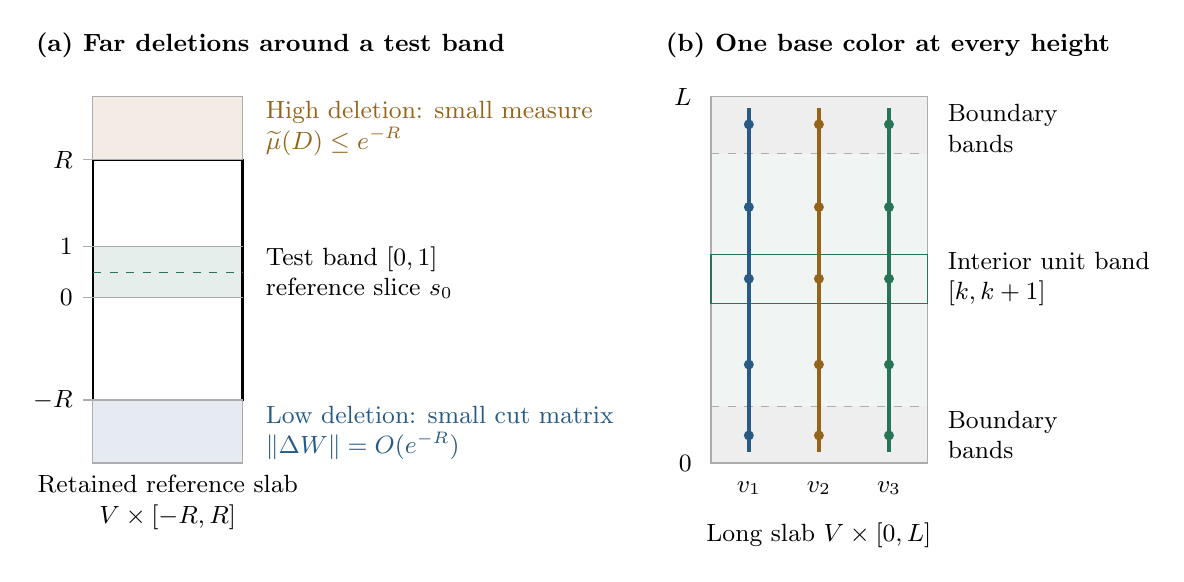
\begin{tikzpicture}[x=1cm,y=1cm,font=\small,
  every node/.style={inner sep=2pt},
  heightline/.style={gray!65,thin},
  fiber/.style={very thick}]
  \definecolor{mahblue}{RGB}{39,91,134}
  \definecolor{mahgold}{RGB}{149,100,27}
  \definecolor{mahgreen}{RGB}{39,116,86}

  \node[anchor=west,font=\small\bfseries] at (0,5.7)
    {(a) Far deletions around a test band};
  \fill[mahgold!12] (.8,4.25) rectangle (2.7,5.05);
  \fill[mahblue!12] (.8,.4) rectangle (2.7,1.2);
  \fill[mahgreen!12] (.8,2.5) rectangle (2.7,3.15);
  \draw[heightline] (.8,.4) rectangle (2.7,5.05);
  \draw[thick] (.8,1.2) rectangle (2.7,4.25);
  \foreach \y/\t in {1.2/{-R},2.5/{0},3.15/{1},4.25/{R}} {
    \draw[heightline] (.68,\y)--(2.7,\y);
    \node[anchor=east] at (.62,\y) {$\t$};
  }
  \draw[dashed,mahgreen] (.8,2.82)--(2.7,2.82);
  \node[anchor=west,align=left,text=mahgold] at (2.92,4.65)
    {High deletion: small measure\\$\widetilde\mu(D)\leq e^{-R}$};
  \node[anchor=west,align=left] at (2.92,2.82)
    {Test band $[0,1]$\\reference slice $s_0$};
  \node[anchor=west,align=left,text=mahblue] at (2.92,.78)
    {Low deletion: small cut matrix\\$\|\Delta W\|=O(e^{-R})$};
  \node[align=center] at (1.75,-.1)
    {Retained reference slab\\$V\times[-R,R]$};

  \node[anchor=west,font=\small\bfseries] at (8,5.7)
    {(b) One base color at every height};
  \fill[gray!13] (8.65,.4) rectangle (11.4,1.12);
  \fill[gray!13] (8.65,4.33) rectangle (11.4,5.05);
  \fill[mahgreen!7] (8.65,1.12) rectangle (11.4,4.33);
  \draw[heightline] (8.65,.4) rectangle (11.4,5.05);
  \draw[heightline,dashed] (8.65,1.12)--(11.4,1.12);
  \draw[heightline,dashed] (8.65,4.33)--(11.4,4.33);
  \draw[mahgreen] (8.65,2.43) rectangle (11.4,3.05);
  \foreach \x/\c in {9.13/mahblue,10.02/mahgold,10.91/mahgreen} {
    \draw[fiber,\c] (\x,.54)--(\x,4.91);
    \foreach \y in {.75,1.65,2.74,3.65,4.7}
      \fill[\c] (\x,\y) circle (1.8pt);
  }
  \node[anchor=east] at (8.48,.4) {$0$};
  \node[anchor=east] at (8.48,5.05) {$L$};
  \node[anchor=west,align=left] at (11.58,4.65) {Boundary\\bands};
  \node[anchor=west,align=left] at (11.58,2.74)
    {Interior unit band\\$[k,k+1]$};
  \node[anchor=west,align=left] at (11.58,.76) {Boundary\\bands};
  \node at (9.13,.08) {$v_1$};
  \node at (10.02,.08) {$v_2$};
  \node at (10.91,.08) {$v_3$};
  \node[align=center] at (10.02,-.52)
    {Long slab $V\times[0,L]$};
\end{tikzpicture}
\caption{Height geometry behind Lemmas~\ref{lem:far-deletion}
and~\ref{lem:coherent-choice} (not to scale). High and low deletions
are controlled by different estimates. A color selected on the
reference slice is used at every height above the same base vertex.
Translated interior unit bands compare with the reference slab in
integrated normalized data; the boundary bands have total length at
most $2R+2$. The colored vertical lines are base fibers
$\{v\}\times[0,L]$, not lifted relation orbits.}
\label{fig:maharam}
\end{figure}


\FloatBarrier
\section{Sparse pinning and descent}
\label{sec:pinning}

\subsection{Sparse pinning and removal of unassigned vertices}

We retain the notation and hypotheses of Theorem~\ref{thm:measured-paving}.
In particular, $b>0$ and $r$ satisfy its strict largest-root inequality,
and $K,C$ are the universal constants from
Lemma~\ref{lem:buffered-pin}.  The lifted graph on a slab is always the
restriction of the original enclosing graph, including edges at which a
particular matrix entry happens to vanish.  All distances below refer to
this enclosing graph.

\begin{proposition}\label{prop:sparse-pinning}
For every $\zeta,\eta>0$ and $L_0\geq1$, there are an integer
$L\geq L_0$ and a measurable partition
\[
 V=\mathcal U\sqcup V_1\sqcup\cdots\sqcup V_r
\]
such that $\mu(\mathcal U)<\eta$ and the following holds.  On the
surviving lifted vertices $(V\setminus\mathcal U)\times[0,L]$, let
$T_{\mathrm{col}}^L$ be the restriction of $T$, keeping only entries
between vertices whose basepoints belong to the same $V_i$, and put
\begin{equation}\label{pin:surviving-operator}
 A_L=d^{1/2}(T_{\mathrm{col}}^L-Kb\one)d^{1/2},
 \qquad d_{(v,s)}=e^s.
\end{equation}
Extend $m_u^{\mathrm{surv}}=((A_L)_+)_{uu}$ by zero on the deleted
vertices.  Then
\begin{equation}\label{pin:surviving-cost}
 \frac1L\int_{V\times[0,L]}m_u^{\mathrm{surv}}\,
 d\widetilde\mu(u)<\zeta.
\end{equation}
\end{proposition}

\begin{proof}
We first construct a partial assignment with small mixed-polynomial
cost. Polynomial moments depend on finite graph balls, so sufficiently
sparse simultaneous pins have an additive first-order response except
on an event of quadratic order in the update probability. Approximating
the derivative of the positive-part function controls the error in
that response independently of the number of roots.
Parameters used to select the slab will be specified below.
On a fixed slab $[0,L]$, write
\[
 \Phi=\frac1L\int_{V\times[0,L]}m_u\,d\widetilde\mu(u).
\]
Choose a common spectral support bound $[-B,B]$ for all the finite
principal systems, pin alternatives, and deletion configurations on this
slab, as in Lemma~\ref{lem:slab-limits}.  For $\tau>0$, choose a real
polynomial $P$ such that
\begin{equation}\label{pin:polynomial-approximation}
 P(-B)=0,\qquad
 \int_{-B}^B\abs{P'(x)-\mathbf1_{(0,\infty)}(x)}\,dx\leq\tau.
\end{equation}
For example, approximate the indicated step function first by a
continuous function in $L^1([-B,B])$, then uniformly by a polynomial,
and integrate that polynomial from $-B$.  It follows that
\[
 \sup_{[-B,B]}\abs{P(x)-x_+}\leq\tau.
\]
Define
\[
 m_{P,u}=\int P(x)\,d\gamma_u(x),\qquad
 \Phi_P=\frac1L\int_{V\times[0,L]}m_{P,u}\,d\widetilde\mu(u).
\]
Since $\gamma_u$ is a probability measure and
$\widetilde\mu(V\times[0,L])=1-e^{-L}\leq1$, we have
\begin{equation}\label{pin:cost-approximation}
 \abs{\Phi-\Phi_P}\leq\tau \qquad(L\geq1).
\end{equation}

\paragraph{The response to one buffered pin.}
At an unassigned lifted vertex $u$, consider pinning to a specified color
$i$, increasing its penalty from $bd_u$ to $Kbd_u$ at the same time.
The total polynomial response on its component is
\begin{equation}\label{pin:single-response}
 \begin{split}
 D_P(u)&=\sum_y\bigl(m_{P,y}^{\mathrm{pin}\ u\mathrm{\ to\ }i}
                         -m_{P,y}^{\mathrm{pre}}\bigr)\\
 &=\int_{-B}^B P'(x)
       \bigl(\xi_{h_{u,i}'}(x)-\xi_{h_u}(x)\bigr)\,dx.
 \end{split}
\end{equation}
Here $h_{u,i}'$ denotes the buffered alternative; the prime does not
denote differentiation.  To prove the identity on a finite principal
set, use the fact that the sum of its local spectral probability
measures is the counting measure of the roots.  The pre-pin and
post-pin polynomials have equal degree and the same principal
polynomial with $u$ removed.  Integrating the difference of their root
counts above $x$ against $P'(x)$ gives exactly
\eqref{pin:single-response}.

Put $k=\max\{1,\deg P\}$.  By the locality in
Lemma~\ref{lem:slab-limits}, only vertices at distance at most $k$ from
$u$ contribute to the sum on the first line of
\eqref{pin:single-response}.  Compute in finite balls large enough to
contain these vertices and their relevant neighborhoods.  The local
polynomial moments stabilize, while the functions $\xi$ converge
weak-* on $[-B,B]$.  This proves the identity on infinite components
as well.  Since both $\xi$-functions take values in $[0,1]$ almost
everywhere, \eqref{pin:polynomial-approximation} implies
\begin{equation}\label{pin:single-error}
 \abs{D_P(u)-(\ell_{u,i}'-\ell_u)}\leq\tau.
\end{equation}

\paragraph{One sparse update.}
For a current partial base assignment, choose the prospective colors
$i(v)$ supplied by Lemma~\ref{lem:coherent-choice}, with tolerance
$\tau_0>0$.  The color $i(v)$ is the same at all heights over $v$.
Properly color the distance-$2k$ power of the base graph with finitely
many auxiliary Borel color classes.  The finite Borel coloring fact
used in the proof of Lemma~\ref{lem:far-deletion} applies because this
power still has bounded degree.  Independently for these auxiliary
classes, select a Bernoulli-$\alpha$ indicator, where $0<\alpha<1$.
Every currently unassigned base vertex in a selected class is pinned to
its prospective color, with its penalty buffered, at all heights
simultaneously.

Within a radius-$k$ lifted ball, different vertices project to different
base vertices, and their pairwise base distance is at most $2k$.
They consequently have different auxiliary classes.  The indicators of
all candidate pins affecting the local moment $m_{P,y}$ are therefore
independent.  This assertion uses injectivity of projection within
each lifted orbit; it does not require independent indicators at all
vertices of the base.

If at most one candidate in this local ball is selected, the change in
$m_{P,y}$ is exactly the sum of its selected single-pin responses.  A
ball has at most a fixed finite number $N$ of vertices, so the
probability of two or more selections is at most
$\binom{N}{2}\alpha^2$.  On this event the discrepancy between the
actual change and the sum of single-pin responses is bounded in
absolute value by a constant depending only on $N$ and
$\sup_{[-B,B]}\abs{P}$.  Integrate this estimate and exchange roots
and pin locations using \eqref{slab:mass-transport}.  The result is
\begin{equation}\label{pin:sparse-update}
 \E[\Phi_P^{\mathrm{new}}\mid\mathrm{pre}]
 \leq\Phi_P+
   \frac\alpha L\int_{\mathrm{unassigned}}D_P(u)\,
                  d\widetilde\mu(u)+C_P\alpha^2.
\end{equation}
All the transports here are measurable, uniformly bounded on the
fixed slab, and supported on bounded-radius pairs.  Thus they are
integrable and the signed version of mass transport is applicable.
The constant $C_P$ may depend on the slab, graph and polynomial, but
not on the current assignment, the prospective choices, or $\alpha$.

By Lemma~\ref{lem:coherent-choice},
\eqref{pin:single-error}, and \eqref{pin:cost-approximation},
\eqref{pin:sparse-update} gives
\begin{equation}\label{pin:recurrence}
 \E[\Phi_P^{\mathrm{new}}\mid\mathrm{pre}]
 \leq(1+C\alpha)\Phi_P+
       \alpha\bigl(\tau_0+(1+C)\tau+C_P\alpha\bigr).
\end{equation}
The same $L$ from Lemma~\ref{lem:coherent-choice} works for all partial
base assignments, so this step can be repeated.

\paragraph{Iteration and choice of parameters.}
Start with every vertex unassigned.  The initial cost is $\Phi=0$ by
Lemma~\ref{lem:slab-limits}.  Use fresh independent class indicators at
each step and recalculate the prospective colors from the current
assignment.  Given $S>0$, perform $n=\lceil S/\alpha\rceil$ steps.
For these fixed parameters there are only finitely many possible
histories.  At every node one may choose separately the measurable
prospective-color functions furnished by
Lemma~\ref{lem:coherent-choice}; no selection measurable in an
infinite-dimensional space of assignments is needed.

We have $n\alpha\leq S+1$ and
$(1+C\alpha)^n\leq e^{C(S+1)}$.  Iterating
\eqref{pin:recurrence}, using the initial bound $\Phi_P\leq\tau$,
and then using \eqref{pin:cost-approximation} again yields
\begin{equation}\label{pin:iteration}
 \E\Phi_{\mathrm{final}}
 \leq\tau+e^{C(S+1)}
   \bigl[\tau+(S+1)(\tau_0+(1+C)\tau+C_P\alpha)\bigr].
\end{equation}
If $\mathcal U$ is the final unassigned base set, each still-unassigned
vertex has conditional probability $\alpha$ of being selected at the
next step, regardless of its prospective color.  Therefore
\begin{equation}\label{pin:unassigned-measure}
 \E\mu(\mathcal U)=(1-\alpha)^n\leq e^{-S}.
\end{equation}

Here is an order of choices which makes both expectations small.
First take $S$ so large that $e^{-S}<\eta/4$.  Next take
$\tau_0,\tau>0$ so small that the terms in
\eqref{pin:iteration} not involving $C_P\alpha$ have sum less than
$\zeta/8$.  Choose an integer $L\geq L_0$ using
Lemma~\ref{lem:coherent-choice} for this $\tau_0$.  Now choose $B$ and
$P$ as above, thereby fixing $C_P$.  Finally take $\alpha$ small
enough that the remaining term in \eqref{pin:iteration} is less than
$\zeta/8$.  Thus
\[
 \E\Phi_{\mathrm{final}}<\zeta/4,
 \qquad \E\mu(\mathcal U)<\eta/4.
\]
Both random variables are nonnegative.  By Markov's inequality and a
union bound, some history satisfies simultaneously
\begin{equation}\label{pin:chosen-history}
 \Phi_{\mathrm{final}}<\zeta,
 \qquad\mu(\mathcal U)<\eta.
\end{equation}
Fix such a history.

\paragraph{Removing the unassigned vertices.}
We show that deleting $\mathcal U\times[0,L]$ cannot increase the
integrated positive cost.  Keep the initial and final deletion states
fixed.  For an arbitrary $\vartheta>0$, choose another polynomial $Q$
with
\[
 Q(-B)=0,\qquad
 \int_{-B}^B\abs{Q'(x)-\mathbf1_{(0,\infty)}(x)}\,dx
 \leq\vartheta.
\]
At each intermediate deletion state, extend $m_{Q,y}$ by zero at
vertices that have already been deleted.

For one deletion at $u$, the total pre-minus-post polynomial cost is
\begin{equation}\label{pin:single-deletion}
 \sum_y\bigl(m_{Q,y}^{\mathrm{pre}}-m_{Q,y}^{\mathrm{post}}\bigr)
     =\int_{-B}^B Q'(x)\xi_{h_u}(x)\,dx\geq-\vartheta.
\end{equation}
For finite sets the identity again follows by integrating the
difference of root counts; the boundary term caused by the loss of one
root is $Q(-B)=0$.  The inequality uses $0\leq\xi_{h_u}\leq1$.
The finite-range locality argument used for
\eqref{pin:single-response} proves the identity in an infinite
component.

Partition the set to be deleted into finitely many Borel batches whose
distinct vertices have distance greater than
$2\max\{1,\deg Q\}$ within each batch in the enclosing lifted
graph.  For one batch, at most one deletion affects any local
polynomial moment, so the batch change is exactly the sum of
single-deletion responses in its pre-state.  Mass transport,
\eqref{pin:single-deletion}, and telescoping over the batches show
that the integrated pre-minus-post polynomial cost, divided by $L$,
is at least
\[
 -\vartheta\,
   \frac{\widetilde\mu(\mathcal U\times[0,L])}{L}.
\]
The error is charged once to each deleted vertex; it is not multiplied
by the number of batches.  Intermediate deleted sets need not be
constant in the height variable, since Lemma~\ref{lem:slab-limits}
allows arbitrary deletion configurations in the enclosing slab.

At each endpoint the integrated error between the $Q$-cost and the
positive cost is at most $\vartheta$.  Thus the pre-minus-post
positive cost is at least $-3\vartheta$.  The endpoints are independent
of $Q$ and of the batch decomposition, so letting $\vartheta\downarrow0$
proves the desired monotonicity.

All surviving vertices are now deterministically colored, with penalty
$Kbd_u$.  Their finite mixed polynomial is the characteristic
polynomial of the corresponding restriction of
\eqref{pin:surviving-operator}, so its local measure is the diagonal
spectral probability measure of that operator.  On an infinite
component the same assertion follows from stabilization of polynomial
moments and the common compact spectral support.  Hence the surviving
positive cost is exactly $m_u^{\mathrm{surv}}$.  Monotonicity and
\eqref{pin:chosen-history} give \eqref{pin:surviving-cost}.
\end{proof}

\subsection{Descent from a slab to the base relation}

The next estimate converts the integrated weighted cost into the desired
spectral error on the base. A finite ball with a large eigenvalue forces
a definite positive cost in its lift; mass transport then bounds the
measure of such bad balls. For an integer $k\geq1$, let $N_k$ be a
uniform upper bound for the number of vertices in a radius-$k$ ball of
the base graph.

\begin{lemma}\label{lem:descent}
Fix $\sigma,\beta>0$, and choose a real polynomial $p$ of degree at most
$k\geq1$ such that
\[
 \sup_{x\in[-1,1]}
 \abs{p(x)-(x-(Kb+\sigma))_+^2}\leq\beta.
\]
Suppose a base partial assignment, with unassigned set $\mathcal U$,
and a slab length $L\geq\max\{1,4k\log J\}$ have surviving cost
\[
 \Psi=\frac1L\int_{V\times[0,L]}m_u^{\mathrm{surv}}\,
                         d\widetilde\mu(u),
\]
where $m^{\mathrm{surv}}$ is defined from
\eqref{pin:surviving-operator}.  Complete the base coloring by giving
$\mathcal U$ one additional color, and denote its paved matrix system
by $T_{\mathrm{pav}}$.  Then
\begin{equation}\label{pin:descent-bound}
 \int_V\bigl((T_{\mathrm{pav}}-(Kb+\sigma)\one)_+^2\bigr)_{vv}
                   \,d\mu(v)
 \leq2\beta+\mu(\mathcal U)+\frac{2J^kN_k}{\sigma}\Psi.
\end{equation}
\end{lemma}

\begin{proof}
Put $g(x)=(x-(Kb+\sigma))_+^2$.  Since the paved operator is a
compression by mutually orthogonal color projections, it remains a
self-adjoint contraction; in particular $0\leq g(T_{\mathrm{pav}})
\leq\one$.

For an assigned base vertex $v$, let $B_k(v)$ be its radius-$k$ ball
in the base graph, and let $T_v$ be the finite compression of the paved
matrix to the assigned vertices of this ball.  Polynomial diagonal
moments through degree $k$ at $v$ are unchanged by this compression.
Indeed every walk contributing to such a moment stays within $B_k(v)$,
and edges from assigned to unassigned vertices are zero after paving.
Consequently
\[
 (p(T_{\mathrm{pav}}))_{vv}=(p(T_v))_{vv}.
\]
Let $\mathcal F$ be the measurable set of assigned vertices for which
$\lambda_{\max}(T_v)>Kb+\sigma$.  Measurability follows by finite
matrix evaluation on the Borel balls.  If $v\notin\mathcal F$ is
assigned, then $g(T_v)=0$ and the two polynomial approximation errors
give
\[
 (g(T_{\mathrm{pav}}))_{vv}\leq2\beta.
\]
On $\mathcal F\cup\mathcal U$ its diagonal is at most $1$.  Therefore
\begin{equation}\label{pin:failure-reduction}
 \int_V(g(T_{\mathrm{pav}}))_{vv}\,d\mu(v)
 \leq2\beta+\mu(\mathcal U)+\mu(\mathcal F).
\end{equation}

It remains to bound $\mu(\mathcal F)$.  Set
$I_{\mathrm{int}}=[k\log J,L-k\log J]$.
For $u=(v,s)$ with $s\in I_{\mathrm{int}}$, the entire ball $B_k(v)$
lifts into the slab: the height change along each graph edge has
absolute value at most $\log J$.  Let $Q_u$ project onto the assigned
vertices of this lifted ball.  With $A_L$ as in
\eqref{pin:surviving-operator}, the order inequality $A_L\leq(A_L)_+$
gives, after compression and diagonal congruence,
\begin{equation}\label{pin:positive-upper-bound}
 T_v-Kb\one
 \leq d_{\mathrm{ball}}^{-1/2}Q_u(A_L)_+Q_u
                                  d_{\mathrm{ball}}^{-1/2}.
\end{equation}
The base and lifted finite matrices here are identified up to the
allowed diagonal unitary gauge, which does not affect the inequality
or any diagonal spectral quantities.  The right side is positive.
If $v\in\mathcal F$, its norm is greater than $\sigma$ by
\eqref{pin:positive-upper-bound}, and hence its trace is greater than
$\sigma$.  Equivalently,
\begin{equation}\label{pin:failure-trace}
 \sum_{y\in B_k(u)\ \mathrm{assigned}}
                \frac{m_y^{\mathrm{surv}}}{d_y}>\sigma.
\end{equation}
Here $B_k(u)$ denotes the lift of the base ball, which agrees with the
radius-$k$ enclosing lifted ball at these interior heights.  The
comparison uses only $A_L\leq(A_L)_+$; it does not require positive
part to commute with compression or diagonal congruence.

Integrate \eqref{pin:failure-trace} against $d\mu(v)\,ds/L$ over
$\mathcal F\times I_{\mathrm{int}}$, and enlarge the resulting
nonnegative sum to all interior roots.  Since
$d\mu(v)\,ds=d_u\,d\widetilde\mu(u)$, the resulting integrand is a
sum of $(d_u/d_y)m_y^{\mathrm{surv}}$.  On a radius-$k$ ball,
$d_u/d_y\leq J^k$.  Exchanging roots and targets by
\eqref{slab:mass-transport}, each target $y$ has at most $N_k$
possible roots.  Deleted vertices may be retained as locations for
the enclosing-ball relation, with $m_y^{\mathrm{surv}}=0$ there.
Thus
\[
 \sigma\frac{\abs{I_{\mathrm{int}}}}L\mu(\mathcal F)
 \leq J^kN_k\Psi.
\]
Our lower bound on $L$ ensures
$\abs{I_{\mathrm{int}}}/L\geq1/2$, including the case $J=1$.
We conclude that
\[
 \mu(\mathcal F)\leq\frac{2J^kN_k}{\sigma}\Psi.
\]
Combining this with \eqref{pin:failure-reduction} proves
\eqref{pin:descent-bound}.
\end{proof}

\begin{proof}[Completion of the proof of Theorem~\ref{thm:measured-paving}]
Fix the prescribed $\sigma,\rho>0$.  Choose $\beta>0$ with
$2\beta<\rho/4$, and then choose the polynomial and its degree
$k\geq1$ in Lemma~\ref{lem:descent}.  Thus $N_k$ is fixed before
selecting the slab.  Take
\[
 \eta=\rho/4,\qquad
 \zeta=\frac{\rho\sigma}{8J^kN_k},\qquad
 L_0=\max\{1,4k\log J\}.
\]
Proposition~\ref{prop:sparse-pinning} supplies a partial assignment and
a slab of length at least $L_0$ with
$\mu(\mathcal U)<\eta$ and $\Psi<\zeta$.  Give $\mathcal U$ the
additional color and apply Lemma~\ref{lem:descent}.  Its right side is
strictly less than $\rho$, as required.

Only the $r$ assigned colors and one extra color occur in the final
partition.  The auxiliary graph colors, the slab length, the
approximation degrees and the number of updates affect its
construction but not this number of final colors.  In particular the
graph and cocycle bounds do not enter the condition on $r$ in the
theorem.
\end{proof}

\section{Expected maximal abelian subalgebras}
\label{sec:expected}

We now combine the measured paving theorem with a separate argument for the
part of an operator orthogonal to the normalizer algebra. Throughout this
section, $M$ has separable predual, $\varphi$ is a faithful normal state, and
$A\subset M$ is a MASA contained in the centralizer $M_\varphi$. We write
$E_A$ for the $\varphi$-preserving normal conditional expectation and use
the sequence quotient of Lemma~\ref{lem:sequence-quotient}. Brackets denote
classes in that quotient; a fixed operator also denotes its constant
sequence. A partition in the quotient will always be represented by
partitions in $A$ with one fixed finite number of members.

\begin{theorem}\label{thm:state-paving}
For every $\gamma>0$ there is an integer $R_{\mathrm{st}}(\gamma)$ with the following
property. For every self-adjoint $x\in M$ with $\norm{x}\leq1$, there are
partitions $\mathcal P_j$ of $1$ in $A$, each with $R_{\mathrm{st}}(\gamma)$ members,
and self-adjoint $w_j\in M$ such that
\begin{equation}\label{exp:state-paving}
 \norm{w_j}\leq2,\qquad
 \norm{w_j}_\varphi\longrightarrow0,\qquad
 \norm{C_{\mathcal P_j}(x-w_j)-E_A(x)}\leq\gamma.
\end{equation}
The integer $R_{\mathrm{st}}(\gamma)$ is independent of $M,A,\varphi$, and $x$.
\end{theorem}

\subsection{The normalizer algebra}

Let $N$ be the von Neumann algebra generated by the groupoid normalizers
of $A$ in $M$. These are the partial isometries $v$ with $v^*v,vv^*\in A$
such that conjugation by $v$ carries $A v^*v$ onto $A vv^*$. The algebra
$N$ contains $A$. Since the modular group of $\varphi$ fixes $A$
pointwise, it carries every groupoid normalizer to another with the same
supports and the same induced corner isomorphism. Hence $N$ is globally
modular invariant. Takesaki's theorem~\cite{Takesaki72} gives a normal
$\varphi$-preserving conditional expectation $E_N:M\to N$; uniqueness of
the state-preserving expectation onto $A$ gives
\begin{equation}\label{exp:expectation-composition}
 E_A E_N=E_A.
\end{equation}

The inclusion $A\subset N$ is Cartan. For completeness, groupoid
regularity here implies regularity by unitary normalizers. Represent $A$
on a standard probability space. A normal isomorphism between two
corners of $A$ is represented by a nonsingular measurable partial
bijection. On its fixed-point set, the corresponding partial normalizer
belongs to $A$. On the complement, a countable separating family of
measurable sets partitions the domain into countably many pieces on each
of which the domain and range are disjoint. If $v$ is the restriction to
one such piece, then
\[
 v+v^*+1-v^*v-vv^*
\]
is a unitary normalizer. Multiplication by its source projection recovers
$v$, and strong summation recovers the original partial normalizer.
Also $A$ is a MASA in $N$ and $E_A|_N$ is a faithful normal expectation,
as required for the Cartan theorem.

The Feldman--Moore representation~\cite{FM77} identifies $A$ with
$L^\infty(V,\mu)$, where $\mu$ is the probability measure given by
$\varphi|_A$, and identifies $N$ with the algebra of a countable
nonsingular equivalence relation, allowing a scalar unitary cocycle.
We use the representation on square-integrable columns, with the right
base point integrated against $\mu$ and counting measure in its orbit.
An algebra element acts by left matrix multiplication on the orbit
column. In the twisted case, changing the base point changes the matrix
by diagonal unitary conjugacy, by the scalar cocycle identity. The
conditional expectation onto $A$ is its rooted diagonal. This is
$E_A|_N$: if $F:N\to A$ is any normal conditional expectation,
bimodularity gives $F(C_{\mathcal Q}(z))=F(z)$. The bounded
compression net converges ultraweakly to $E_A(z)$ by
Lemma~\ref{lem:compression-net}, so normality gives
$F(z)=F(E_A(z))=E_A(z)$.

Bounded graph partial-isometry kernels and diagonal coefficients generate
$N$. Their algebraic span, including products, is strongly dense. A
finite such expression has off-diagonal support in a finite union of
partial-bijection graphs, and therefore in an undirected graph of
uniformly bounded degree. Operator-norm bounds in the column
representation give the same matrix bounds for almost every orbit. All
models and cocycle identities below may be restricted to a common
conull invariant set for the countably many operators involved.

Fix $x=x^*$ with $\norm{x}\leq1$, and put
\begin{equation}\label{exp:decomposition}
 a_0=E_Ax,\qquad Y=E_Nx-a_0,\qquad Z=x-E_Nx.
\end{equation}
Then $x-a_0=Y+Z$, with $\norm{Y},\norm{Z}\leq2$ and $E_NZ=0$.
The measured theorem will control $Y$ through its relation matrices.
For $Z$, a unitary dilation with a diffuse left--right kernel will provide
random diagonal compressions whose moments approach a free compression law. Its norm
bound will make the spectral excess state-null, giving a second
quotient norm estimate. Common refinement combines the two bounds;
clipping the resulting block-diagonal residual then supplies the
correction in Theorem~\ref{thm:state-paving}.

\begin{lemma}\label{exp:normalizer-paving}
Let $b,\sigma>0$ and let $r$ be an integer such that
\[
 2\sqrt{2/r}+2/r<b.
\]
There are sequences of $A$-partitions with $(r+1)^2$ members whose
quotient partition $\mathcal P$ satisfies
\begin{equation}\label{exp:normalizer-bound}
 \norm{C_{\mathcal P}[Y]}\leq6(Kb+\sigma),
\end{equation}
where $K$ is the universal constant in
Theorem~\ref{thm:measured-paving}.
\end{lemma}

\begin{proof}
Bounded Kaplansky approximation, followed by norm approximation inside
the generating algebra, gives self-adjoint finite graph expressions
converging strongly-star to $Y$, with norms at most $3$. Subtracting
their $A$-expectations makes their diagonals zero and increases the norm
bound to $6$; state-norm contractivity of $E_A$ preserves convergence.
For each such expression, cut down by the base set on which every
incident edge in its finite-degree enclosing graph has cocycle ratio
between $J^{-1}$ and $J$. These sets increase to full measure as
$J\to\infty$, and the cuts converge strongly-star to the expression.
A diagonal choice therefore gives self-adjoint $Y_j$ with
\[
 E_AY_j=0,\qquad \norm{Y_j}\leq6,\qquad
 \norm{Y_j-Y}_\varphi^\#\longrightarrow0,
\]
whose orbit matrices have bounded-degree support and bounded cocycle
ratios, with the bounds allowed to depend on $j$.

Apply Theorem~\ref{thm:measured-paving} to $Y_j/6$ and separately to
$-Y_j/6$, using state-error tolerances tending to zero. The rooted
diagonal formula for the state says that the positive part above
$Kb+\sigma$ has $\varphi$-norm tending to zero in each case. These
positive parts are self-adjoint and uniformly bounded, so they belong
to the null ideal of Lemma~\ref{lem:sequence-quotient}. The sequence
$Y_j-Y$ belongs to that ideal as well. The resulting two quotient
partitions, each of size $r+1$, therefore give respectively
\[
 C_{\mathcal P^+}[Y/6]\leq(Kb+\sigma)1,
 \qquad
 C_{\mathcal P^-}[Y/6]\geq-(Kb+\sigma)1.
\]
Take their common refinement. All partition projections commute, and
compression is positive and unital, so both scalar bounds hold after
refinement. This proves the lemma. Further finite $A$-refinement
preserves the bound.
\end{proof}

We have completed the normalizer part. The remaining component has the
following target, whose proof is given after the kernel and free-moment
lemmas below.

\begin{proposition}\label{prop:off-normalizer}
For every $n\geq2$, there are sequences of $n$-partitions in $A$
whose quotient partition $\mathcal P$ satisfies
\begin{equation}\label{exp:off-normalizer-bound}
 \norm{C_{\mathcal P}[Z]}\leq\frac4{\sqrt n}.
\end{equation}
\end{proposition}

\subsection{The diffuse kernel outside the normalizer algebra}
We retain the faithful normal state $\varphi$, with $A\subset M_\varphi$,
and the algebra $N$ generated by the groupoid normalizers of $A$.
Use a standard probability model $A=L^\infty(V,\mu)$ for
$\varphi|_A$.  We use the standard-form realization $L^2(M)$, equivalently
Haagerup $L^2(M)$, and write $\varphi^{1/2}$ for the positive vector
implementing $\varphi$.  In particular,
$a\varphi^{1/2}=\varphi^{1/2}a$ for $a\in A$.

For $X\in M$, the commuting left and right actions of $A$ give a finite
joint spectral measure $\nu_X$ for $X\varphi^{1/2}$ on $V\times V$.
Our first coordinate is the right coordinate: for Borel sets $B,C\subset V$,
\begin{equation}\label{exp:joint-measure}
 \nu_X(B\times C)
 =\big\|1_CX\varphi^{1/2}1_B\big\|_2^2
 =\int_B E_A(X^*1_CX)(v)\,d\mu(v).
\end{equation}
Both marginal measures are absolutely continuous with respect to $\mu$.
The right marginal has density $E_A(X^*X)\leq\|X\|^2$; the left marginal
is absolutely continuous because $a\mapsto\varphi(X^*aX)$ is normal on
$A$.  Disintegration on standard Borel spaces therefore gives a measurable
kernel $k_X(v,dw)$ such that
\begin{equation}\label{exp:kernel}
 \nu_X(dv,dw)=d\mu(v)k_X(v,dw),\qquad
 E_A(X^*aX)(v)=\int_V a(w)\,k_X(v,dw),\qquad
 k_X(v,V)\leq\|X\|^2
\end{equation}
almost everywhere, for $a\in A$.  As usual, individual function identities
are understood modulo null sets.  The joint spectral resolution can be
constructed from a bounded real coordinate generating the standard model
and the commuting left and right spectral resolutions of that coordinate.

\begin{lemma}\label{lem:atomless}
 If $E_N(X)=0$, then $k_X(v,\cdot)$ has no atoms for almost every $v\in V$.
\end{lemma}

\begin{proof}
Choose Borel representatives for the kernel.  The set
\[
 \mathcal T=\{(v,w):k_X(v,\{w\})>0\}
\]
is Borel and has countable sections in the second coordinate.  For example,
joint measurability of the singleton mass follows by using shrinking
neighborhoods in a compatible separable metric on the standard Borel
space.  The countable-section uniformization theorem expresses
$\mathcal T$ as a countable union of graphs of partial Borel maps.
If the conclusion fails, one such map $F:S\to V$ has a domain of positive
$\mu$-measure, with
\[
 g(v):=k_X(v,\{F(v)\})>0\quad(v\in S).
\]
There is no assumption that $F$ is injective.  For a $\mu$-null Borel set
$B\subset V$, absolute continuity of the left marginal gives
\[
 \int_{S\cap F^{-1}(B)}g(v)\,d\mu(v)
 \leq\nu_X(V\times B)=0.
\]
Thus $F$ pulls back null sets to null sets.  With $e=1_S\in A$, composition
with $F$ consequently defines a normal $*$-homomorphism
\[
 \theta:A\longrightarrow Ae,\qquad
 \theta(a)(v)=a(F(v))\quad(v\in S),\qquad \theta(1)=e.
\]
The graph will intertwine $A$ with the possibly proper subalgebra
$\theta(A)$ of $Ae$; its polar partial isometry need not yet normalize
$A$. We will use an expected type I intermediate algebra to split the
right support into corners where these two abelian algebras coincide.

Apply the joint spectral projection of the graph of $F$ to
$X\varphi^{1/2}$ and call the resulting vector $\zeta$.  It is nonzero and
satisfies
\begin{equation}\label{exp:graph-intertwining}
 \zeta e=\zeta,\qquad a\zeta=\zeta\theta(a)\quad(a\in A).
\end{equation}
Its right spectral density on $S$ is $g$.  In particular, $e$ is its
smallest right supporting projection among the projections of $A$:
if $f\in A$ is a projection and $\zeta f=\zeta$, then $e\leq f$.

Take the $L^2$ polar decomposition
$\zeta=u h$, where $h=|\zeta|\in L^2(M)_+$ and $u\in M$ is a partial
isometry.  Put $p=u^*u\leq e$ and $q=uu^*$.  We use here the usual
polar decomposition and support properties of standard-form
noncommutative $L^2$; see, for example, \cite[Lemma~11.12 and Theorem~11.30]{Hiai20}.
For a unitary $a\in A$, the operator $b=\theta(a)+1-e$ is unitary and
\eqref{exp:graph-intertwining} reads $a\zeta=\zeta b$.
Taking absolute values gives $h=b^*hb$.  Uniqueness of the polar
decomposition then gives $au=ub=u\theta(a)$.  Consequently,
\begin{equation}\label{exp:polar-intertwining}
 h\theta(a)=\theta(a)h,\qquad
 p\theta(a)=\theta(a)p,\qquad
 au=u\theta(a)\quad(a\in A),\qquad q\in A.
\end{equation}
The identities for all $a$ follow by linearity from unitaries.  For the
last assertion, the identities imply that $q$ commutes with $A$, and $A$
is maximal abelian.

Consider the von Neumann algebra
\[
 D=\theta(A)'\cap eMe.
\]
It contains $p$ and $Ae$, and $Ae$ is a MASA in $D$.
Moreover $\theta(A)\subset Z(D)$.  If $d\in pDp$, then $udu^*$ commutes
with $Aq$, by \eqref{exp:polar-intertwining}, and hence belongs to $Aq$.
On the other hand,
\[
 u\theta(a)p u^*=aq\quad(a\in A).
\]
Conjugation by $u$ therefore identifies $pDp$ with $Aq$, and
\begin{equation}\label{exp:abelian-corner}
 pDp=\theta(A)p.
\end{equation}
Let $c$ be the central support of $p$ in $D$.  Since
$Z(D)\subset Ae$, the identity $pc=p$ gives $\zeta c=\zeta$; the minimal
right $A$-support property gives $c=e$.  Thus $D$ has an abelian projection
with full central support and is type I.  Finally, if $d\in Z(D)$, then
\eqref{exp:abelian-corner} gives $dp=\theta(a)p$ for some $a\in A$.
The central element $d-\theta(a)$ annihilates a projection of full central
support and is zero.  We have proved
\begin{equation}\label{exp:center}
 Z(D)=\theta(A).
\end{equation}

We next need a partition of $e$ by projections $e_j\in Ae$ such that
\begin{equation}\label{exp:branch-partition}
 (Ae)e_j=\theta(A)e_j.
\end{equation}
The restriction of $E_A$ to $D$ is a normal conditional expectation onto
$Ae$.  The type I MASA theorem of Akemann and Sherman
\cite[Theorem~4.1]{AS12} supplies a partition of $e$ by projections in
$Ae$ that are abelian in $D$.  There are only countably many nonzero
members, because $D$ has the faithful normal state
$\varphi|_D/\varphi(e)$.  For an abelian projection in a type I algebra,
\[
 e_jDe_j=Z(D)e_j.
\]
This follows, for instance, by writing the type I algebra as a direct
integral: an abelian projection has fiber rank at most one.  Together
with \eqref{exp:center} and $\theta(A)\subset Ae\subset D$, this proves
\eqref{exp:branch-partition}.

Set $\eta_j=\zeta e_j$ and take its polar decomposition
$\eta_j=u_j h_j$.  Its right support is at most $e_j$.  Repeating
\eqref{exp:polar-intertwining} shows that $h_j$ commutes with $\theta(A)$
and that
\[
 au_j=u_j\theta(a)\quad(a\in A).
\]
By \eqref{exp:branch-partition} and the support condition, $h_j$ commutes
with all of $A$.  Therefore the right support $p_j=u_j^*u_j$ belongs to
$A$; the left support $q_j=u_ju_j^*$ belongs to $A$ by the same polar
argument as before.  In addition,
\[
 \theta(A)p_j=Ap_j,\qquad
 u_j(Ap_j)u_j^*=Aq_j.
\]
Thus each nonzero $u_j$ is a groupoid normalizer and belongs to $N$.

Let $\psi_j$ be the normal positive functional whose positive
implementing vector is $h_j$.  Since $h_j$ commutes with $A$, this
functional centralizes $A$.  In particular
$\psi_j\circ C_{\mathcal Q}=\psi_j$ for every finite partition
$\mathcal Q$ in $A$.  Lemma~\ref{lem:compression-net}, normality, and
boundedness of the compression net imply
\[
 \psi_j=\psi_j\circ E_A.
\]
Write $f_j=d(\psi_j|_A)/d\mu\in L^1(V,\mu)_+$ and
$f_{j,m}=\min(f_j,m)$.  The positive vectors
$f_{j,m}^{1/2}\varphi^{1/2}$ belong to $A\varphi^{1/2}$ and converge in
$L^2$; indeed their squared pairwise distances are
\[
 \int_V\big|f_{j,m}^{1/2}-f_{j,n}^{1/2}\big|^2\,d\mu.
\]
Their normal positive functionals are
$x\mapsto\int f_{j,m}E_A(x)\,d\mu$ and converge in norm to $\psi_j$.
The limit is therefore the unique positive implementing vector $h_j$.
It follows that
\[
 h_j\in\overline{A\varphi^{1/2}},\qquad
 \eta_j\in\mathcal H_N:=\overline{N\varphi^{1/2}}.
\]
The right projections $e_j$ are orthogonal and sum to $e$, so
$\zeta=\sum_j\zeta e_j\in\mathcal H_N$, with convergence in $L^2$.

The closed space $\mathcal H_N$ reduces both the left and right actions
of $A$: for the right action, use
$n\varphi^{1/2}a=na\varphi^{1/2}$.  It therefore reduces their joint
spectral projections, including the graph projection defining $\zeta$.
But $E_N(X)=0$ gives, for $n\in N$,
\[
 \varphi(n^*X)=\varphi(n^*E_N(X))=0,
\]
so $X\varphi^{1/2}\perp\mathcal H_N$.  Thus
$\zeta\perp\mathcal H_N$, contradicting $\zeta\ne0$ and the
membership just proved.
\end{proof}

\paragraph{Removing atomic summands.}
For the remaining treatment of $Z=x-E_N(x)$ we may assume that $A$ is
diffuse.  Here are the details of this reduction.  If $f$ is an atom of
$A$, then $Af=\mathbb C f$ is a MASA in $fMf$, so $fMf=\mathbb C f$.
Thus $f$ is minimal in $M$.  Let $z_f$ be its central support in $M$.
The algebra $z_fM$ is type I, since $f$ is an abelian projection with
full central support there.  Compression by $f$ is faithful on its
center and has scalar range, so $z_fM$ is a type I factor.

The algebra $Az_f$ is a MASA in this factor and has the normal
expectation $E_A|_{z_fM}$.  Again by \cite[Theorem~4.1]{AS12}, it has a
partition of $z_f$ into rank-one projections.  In particular it is
purely atomic.  Partial isometries joining any two of these rank-one
projections normalize their $A$-corners.  A compatible system of these
matrix units generates $z_fM$, and hence
\[
 z_fM\subset N.
\]
Distinct central supports of atoms are either equal or orthogonal,
because each supports a factor summand.  Their sum $z_{\mathrm{at}}$ is
a central projection, belongs to $A$, and satisfies
$z_{\mathrm{at}}M\subset N$.  Consequently
\[
 z_{\mathrm{at}}Z=0.
\]
On the complementary central summand, $A(1-z_{\mathrm{at}})$ has no
atoms.  The algebra generated there by its groupoid normalizers is
$N(1-z_{\mathrm{at}})$: corner normalizers extend by zero, and global
normalizers restrict to this central summand.  We may use the normalized
restriction of $\varphi$ on the nonzero complementary summand.  This
changes state seminorms only by a fixed scalar factor.
A partition obtained there extends to $M$ with the same number of cells
by adding $z_{\mathrm{at}}$ to one cell; all estimates for $Z$ are
preserved because $Z$ vanishes on $z_{\mathrm{at}}$.


\subsection{Random diagonal unitaries and free moments}

It remains to compress the diffuse summand of $Z$.
The next two lemmas supply the free law and its norm bound for the
matrix dilation used to prove Proposition~\ref{prop:off-normalizer}.
The state in the probabilistic argument need not be tracial.

\begin{lemma}\label{lem:random-freeness}
Let $\mathcal M$ have separable predual, let $\phi_0$ be a faithful
normal state, and let $D\subset\mathcal M_{\phi_0}$ be a diffuse MASA.
Suppose that $U\in\mathcal M$ is a self-adjoint unitary with
$\phi_0(U)=0$, and that the normal positive map
\[
 \mathcal K(a)=E_D(UaU),\qquad a\in D,
\]
has an almost everywhere diffuse kernel on a standard probability
model of $(D,\phi_0|_D)$. For every integer $n\geq2$ there are unitaries
$w_l\in D$, with $w_l^n=1$, such that the joint star moments of
$(w_l,U)$ converge to those of free unitaries $(w,U_{\mathrm f})$,
where $w$ is uniform on the $n$th roots of unity and $U_{\mathrm f}$
is uniform on $\{-1,1\}$.
\end{lemma}

\begin{proof}
Choose an increasing sequence of finite partitions $\mathcal Q$ in
$D$ which generates $D$, separates points of a conull standard model,
and satisfies
\begin{equation}\label{exp:small-cells}
 \max_{q\in\mathcal Q}\phi_0(q)\longrightarrow0.
\end{equation}
Such a sequence is obtained by adjoining a countable separating family
and, at each stage, a sufficiently small-mass finite refinement; the
latter exists by diffuseness. Give its cells independent labels $Z_q$
uniform on the $n$th roots of unity, and put $w_{\mathcal Q}=\sum_q Z_q q$.

We first make the averaged reduced moments vanish by estimating return
probabilities for diffuse kernels. We then control their fluctuations
using the small masses of the partition cells, so that one deterministic
labeling works for each prescribed finite list of moments.

\paragraph{Averaged words and a repeated-cell compression.}
We first prove that the label expectation tends to zero for each scalar
\begin{equation}\label{exp:reduced-test-word}
 F_{\mathcal Q}
 =\phi_0(x_0 w_{\mathcal Q}^{k_1}x_1\cdots
                 w_{\mathcal Q}^{k_h}x_h),
 \qquad h\geq1,\quad 1\leq k_j<n,
\end{equation}
where $x_j=U$ for $1\leq j<h$ and each endpoint $x_0,x_h$ is either
$1$ or $U$. Expand over cell assignments $q_1,\ldots,q_h$.
An assignment survives label averaging only if, in every block of equal
cells, the sum of its exponents is zero modulo $n$. Consequently every
block of its exact equality pattern has size at least two. For any
surviving exact pattern, inclusion-exclusion expresses its word sum as
a finite linear combination of sums
\begin{equation}\label{exp:partition-word-sum}
 S_\pi
 =\sum_{\substack{q_1,\ldots,q_h\in\mathcal Q\\
                    q_i=q_j\text{ if }i,j\text{ are in one block of }\pi}}
      \phi_0(x_0q_1x_1\cdots q_hx_h),
\end{equation}
where every block of $\pi$ has at least two members. There is no
distinctness requirement between different blocks in
\eqref{exp:partition-word-sum}. It is enough to show $S_\pi\to0$ for
each such $\pi$.

Choose positions $c<d$ in one block whose distance $d-c$ is minimal
among all pairs in a common block. The positions strictly between them
belong to distinct other blocks. We impose the equalities of $\pi$
using auxiliary Haar phases. For a block other than the selected block,
place independently sampled cellwise Haar diagonal unitaries at all
but one of its occurrences, and their inverse product at the remaining
occurrence. Haar averaging forces precisely the equality of the cells
at those occurrences. In the selected block, use the same projection
$q$ explicitly at $c$ and $d$ and sum over $q$; put independent Haar
diagonals at every other occurrence of that block, with their inverse
product additionally at $c$. All initial draws are independent.
Expanding and averaging now gives exactly $S_\pi$ as the auxiliary
expectation of
\begin{equation}\label{exp:haar-compression}
 \phi_0\bigl(\mathrm{PRE}\,C_{\mathcal Q}(Y_{\mathcal Q})\,
                    \mathrm{POST}\bigr),\qquad
 Y_{\mathcal Q}=U d_{c+1}U\cdots d_{d-1}U.
\end{equation}
When $d=c+1$, the last expression is $U$. The extra inverse product at
$c$ can be moved before its projection, since both lie in $D$, and is
included in $\mathrm{PRE}$. The factors outside the compression are
products of fixed contractions $x_j$ and diagonal unitaries. Each
interior $d_j$ is a cellwise Haar diagonal: this is also true if it is
the inverse product placed at the last occurrence of its block. The
interior diagonals are mutually independent because their positions
belong to different blocks. Independence from $\mathrm{PRE}$ and
$\mathrm{POST}$ is not asserted or needed.

Their independence and orthogonality of the outside projections give
\begin{equation}\label{exp:haar-square-sum}
 \E\norm{C_{\mathcal Q}(Y_{\mathcal Q})}_{\phi_0}^2
 =\sum_{q,q_{c+1},\ldots,q_{d-1}\in\mathcal Q}
   \norm{qUq_{c+1}U\cdots q_{d-1}Uq}_{\phi_0}^2.
\end{equation}
There are no middle cells when $d=c+1$. Fix a coarser partition
$\mathcal E$ from the generating sequence. When $\mathcal Q$ refines
$\mathcal E$, contractivity of $C_{\mathcal Q}$ in the state norm,
applied with each middle cell tuple fixed, bounds the right side by
\begin{equation}\label{exp:coarse-square-sum}
 \sum_{p\in\mathcal E}
 \sum_{q_{c+1},\ldots,q_{d-1}\in\mathcal Q}
   \norm{pUq_{c+1}U\cdots q_{d-1}Up}_{\phi_0}^2.
\end{equation}

\paragraph{Diffuse kernel return probabilities.}
Here is the limit of this expression without a tracial assumption.
Put $m=d-c$. For each $p\in\mathcal E$ define
\[
 B_{1,\mathcal Q}(p)=UpU,\qquad
 B_{j+1,\mathcal Q}(p)=U C_{\mathcal Q}(B_{j,\mathcal Q}(p))U.
\]
Expanding the squares in \eqref{exp:coarse-square-sum} and summing the
middle cells identifies that expression with
$\sum_{p\in\mathcal E}\phi_0(pB_{m,\mathcal Q}(p)p)$.
All $B_{j,\mathcal Q}(p)$ are positive contractions. By
Lemma~\ref{lem:compression-net}, $C_{\mathcal Q}(t)\to E_D(t)$
strongly-star on each fixed bounded element. Its contractivity for
both state seminorms also controls a bounded, varying, strong-star
null error. Bounded strong-star continuity of multiplication by the
fixed $U$ therefore proves recursively that $B_{j,\mathcal Q}(p)$
converges strongly-star to $B_j(p)$, where
\[
 B_1(p)=UpU,\qquad B_{j+1}(p)=U E_D(B_j(p))U.
\]
Thus $E_D(B_j(p))=\mathcal K^j(p)$. If $\mu_0$ denotes the probability
measure on $D$, state preservation and bimodularity of $E_D$ show that
the limit of \eqref{exp:coarse-square-sum} is
\begin{equation}\label{exp:kernel-return}
 \sum_{p\in\mathcal E}\phi_0(p\mathcal K^m(p)p)
 =\sum_{p\in\mathcal E}\int_p(\mathcal K^m1_p)(v)\,d\mu_0(v).
\end{equation}

The positive normal map $\mathcal K$ is unital. Its kernel is
nonsingular in the integrated sense: a fixed $\mu_0$-null set receives
zero mass for almost every starting point. This follows from
normality, since its indicator is zero in $D$. In particular the
kernel avoids, for almost every starting point, the fixed exceptional
null set on which its successor kernel is not diffuse. Integrating
diffuse successor kernels consequently produces a diffuse kernel.
Induction shows that each fixed iterate $\mathcal K^m$ has an almost
everywhere diffuse kernel. As $\mathcal E$ increases along the
separating sequence, the cell containing $v$ decreases to $\{v\}$ on
the chosen conull model. Its return mass in
\eqref{exp:kernel-return} therefore tends to zero for almost every
$v$. It is bounded by $\mathcal K^m1(v)=1$. Dominated convergence
proves that \eqref{exp:kernel-return} tends to zero. First fixing
$\mathcal E$ and letting $\mathcal Q$ refine, and then letting
$\mathcal E$ refine, proves
\begin{equation}\label{exp:haar-square-zero}
 \E\norm{C_{\mathcal Q}(Y_{\mathcal Q})}_{\phi_0}^2\longrightarrow0.
\end{equation}

\paragraph{Nontracial state estimates.}
We next explain the state estimates that turn this into scalar moment
convergence. For an entire analytic element $a$ for the modular group,
the standard-form right-action identity gives
\begin{equation}\label{exp:analytic-right}
 \norm{ta}_{\phi_0}
 \leq\norm{\sigma_{i/2}^{\phi_0}(a)}\norm{t}_{\phi_0}.
\end{equation}
See \cite[Lemma~8.12, Equation~(8.4)]{Hiai20}, applied to $a^*$.
Entire analytic elements approximate each fixed element boundedly in
the state norm, for example by Gaussian modular smoothing
\cite[Lemma~2.13]{Hiai20}. A centralizer unitary has right-multiplication bound
$1$. In any scalar word consisting of fixed bounded factors and
varying centralizer unitaries, replace the fixed factors from right to
left by bounded analytic approximants. At a replacement step all
factors to the right already have uniformly bounded right actions,
and all factors to the left have uniformly bounded operator norms.
The error in the scalar state value is therefore at most a fixed
constant times the state-norm error of the factor being replaced.
Choosing the approximants in that order makes the total error
arbitrarily small, uniformly over the varying diagonals and
partitions.

Apply this procedure only to the fixed factors in $\mathrm{POST}$
in \eqref{exp:haar-compression}. The compression and all remaining
left factors are contractions. With the approximants fixed, the
absolute scalar value is bounded by
$C\norm{C_{\mathcal Q}(Y_{\mathcal Q})}_{\phi_0}$, where $C$ is
independent of every phase and of $\mathcal Q$. Cauchy--Schwarz in
the auxiliary probability space and \eqref{exp:haar-square-zero}
make its phase expectation tend to zero. The uniformly arbitrarily
small replacement error proves $S_\pi\to0$. Hence
\begin{equation}\label{exp:word-expectation-zero}
 \E F_{\mathcal Q}\longrightarrow0.
\end{equation}

\paragraph{Concentration and deterministic labels.}
It remains to choose deterministic labels simultaneously for the
moments. Replace all fixed factors in
\eqref{exp:reduced-test-word} analytically, again from right to left,
and call the resulting scalar $G_{\mathcal Q}$. It approximates
$F_{\mathcal Q}$ uniformly to any prescribed accuracy. Changing one
label $Z_q$ changes a power of $w_{\mathcal Q}$ by a scalar of
absolute value at most $2$ times $q$. Telescoping over the finitely
many occurrences, each difference is thus a bounded scalar times
$\phi_0(\mathrm{PRE}\,q\,\mathrm{POST})$. Cauchy--Schwarz gives
\begin{align}\label{exp:two-sided-influence}
 \abs{\phi_0(\mathrm{PRE}\,q\,\mathrm{POST})}
 &\leq\norm{q\mathrm{PRE}^*}_{\phi_0}
        \norm{q\mathrm{POST}}_{\phi_0}\notag\\
 &\leq C_{\mathrm{word}}\phi_0(q).
\end{align}
The second line follows from \eqref{exp:analytic-right} for both
products, including their analytic adjoints. Their modular norm
bounds are uniform over all other labels, since the diagonal
unitaries are in the centralizer. Independent bounded differences
(or the martingale variance sum obtained by revealing one label at
a time) now give
\[
 \E\abs{G_{\mathcal Q}-\E G_{\mathcal Q}}^2
 \leq C'_{\mathrm{word}}\sum_{q\in\mathcal Q}\phi_0(q)^2
 \longrightarrow0
\]
by \eqref{exp:small-cells}. The uniform approximation shows that
$F_{\mathcal Q}-\E F_{\mathcal Q}\to0$ in probability. Together with
\eqref{exp:word-expectation-zero}, this gives
$F_{\mathcal Q}\to0$ in probability.

There are only countably many test words. For successively larger
finite lists, convergence in probability gives a partition far
enough along the sequence and a deterministic labeling for which
every word in the list is as small as prescribed. A diagonal choice
gives $w_l$ with all those moments tending to zero. The tests include
the nontrivial single powers of $w_l$, so its limiting distribution
is uniform on the $n$th roots. Also $U^2=1$ and $\phi_0(U)=0$ give
the symmetric two-point distribution. Centered elements of the two
limiting generated algebras are linear combinations of the tested
powers and of $U$, respectively; all alternating centered moments
are precisely the tests above. This establishes the asserted joint
free law.
\end{proof}

\begin{lemma}\label{lem:free-compression}
Let $w$ and $U_{\mathrm f}$ have the free law in
Lemma~\ref{lem:random-freeness}, in its reduced free-product
representation. If $p_1,\ldots,p_n$ are the spectral projections of
$w$, then
\begin{equation}\label{exp:free-norm-bound}
 \norm{\sum_{j=1}^n p_j U_{\mathrm f}p_j}\leq\frac2{\sqrt n}.
\end{equation}
\end{lemma}

\begin{proof}
Let $E_0$ be the Hilbert-space projection onto the vacuum and all
reduced words not starting in the centered part of the $w$-algebra.
For a spectral projection $p$ of $w$, put $t=1/n$. On this subspace,
left multiplication by $p$ is the sum of the scalar action $t$ and
creation by $p-t1$. The two resulting subspaces are orthogonal, and
$\norm{p-t1}_2^2=t(1-t)$; hence
\[
 \norm{pE_0}=\norm{E_0p}=\sqrt{t}.
\]
Since $U_{\mathrm f}$ is centered, it sends a word starting in the
$w$-centered space to a word starting in the other factor. Therefore
$U_{\mathrm f}(1-E_0)=E_0U_{\mathrm f}(1-E_0)$, and
\[
 pU_{\mathrm f}p
 =pU_{\mathrm f}E_0p+pE_0U_{\mathrm f}(1-E_0)p.
\]
Unitarity gives norm at most $2\sqrt t$. The sum of the compressions
is block diagonal for the mutually orthogonal $p_j$, so its norm is
the largest block norm.
\end{proof}

\subsection{A free-product matrix dilation}

\begin{proof}[Proof of Proposition~\ref{prop:off-normalizer}]
By the atomic reduction following Lemma~\ref{lem:atomless}, it is
enough to work on the central summand where $A$ is diffuse. Normalize
the state on that summand and retain the same notation. Put $z=Z/2$,
so $z$ is a self-adjoint contraction and $E_Nz=0$.

The ordinary two-by-two unitary dilation need not have a diffuse
kernel over $A\oplus A$: already at $z=0$, its identity off-diagonal
entry gives an atomic cross-kernel. We replace the second diagonal
algebra by a free diffuse abelian algebra, turning the cross terms
into normal functionals on diffuse spaces. This is the symmetry form
of the free-product projection dilation in
\cite[proof of Theorem~5.1]{PV15}: with $y=(1+z)/2$, the symmetry
below is twice that projection minus the identity. The kernel and
moment lemmas above supply the required freeness in the present
nontracial setting.

Let $(B_0,\tau_B)$ be a diffuse standard separable abelian probability
algebra and form the reduced von Neumann free product
\[
 (P,\psi)=(M,\varphi)*(B_0,\tau_B).
\]
The free-product state is faithful and normal, the two factor
expectations preserve it, and its Hilbert-space representation is
the reduced-word representation; see, for example,~\cite{HU}.
Both $A$ and $B_0$ remain MASAs in $P$. We give the argument to
make its nontracial applicability explicit. There are unitaries
$v_k\in A$ tending weakly to zero, since $A$ is diffuse. They
centralize $\psi$, by the expectation onto $M$. On
$L^2(P,\psi)\ominus L^2(M,\varphi)$, a dense family consists of
vectors of words
\[
 x_0 b_1 x_1\cdots b_hx_h,\qquad h\geq1,
\]
where $b_i\in B_0$ are centered, the internal $x_i\in M$ are
centered, and the endpoints are arbitrary. To compute a matrix
coefficient of conjugation by $v_k$, take another such word with
initial endpoint $y_0$, and split the middle product
$y_0^*v_kx_0$ into its centered part and its scalar mean. The
centered part gives a reduced word with zero expectation onto $M$.
The scalar part is $\varphi(y_0^*v_kx_0)$ times an expression with
a fixed norm bound and tends to zero. The additional right factor
$v_k^*$ in the conjugation does not change that norm bound.
Conjugation is unitary on the state Hilbert space; density proves
that it tends weakly to zero on the indicated complement. If an
element of $P$ commutes with $A$, its vector after subtracting its
$M$-expectation lies in this complement and is fixed by all these
conjugations. It must be zero. The element belongs to $M$, and
then to $A$. Interchanging the factors proves the assertion for
$B_0$.

In $\widetilde M=\operatorname{Mat}_2(P)$ use the state
$\widetilde\varphi=\tr_2\otimes\psi$, with normalized matrix trace.
The diagonal algebra $D=A\oplus B_0$ is a diffuse MASA in its
centralizer. Define
\begin{equation}\label{exp:unitary-dilation}
 U=\begin{pmatrix}z&s\\s&-z\end{pmatrix},\qquad
 s=(1-z^2)^{1/2}.
\end{equation}
Since $z$ commutes with $s$, this is a self-adjoint unitary.
Furthermore $E_D(U)=0$. For $a\in A$ and $b\in B_0$,
direct free-product expectation gives
\begin{equation}\label{exp:dilation-kernel}
 E_D\bigl(U(a\oplus b)U\bigr)
 =\bigl(E_A(zaz)+\tau_B(b)E_A(s^2)\bigr)
  \oplus
  \bigl(\varphi(sas)1+\tau_B(b)\varphi(z^2)1\bigr).
\end{equation}
In particular, $E_{B_0}(zbz)=\tau_B(b)\varphi(z^2)1$ because
$\varphi(z)=0$. Lemma~\ref{lem:atomless} makes the first kernel
$a\mapsto E_A(zaz)$ diffuse. The other kernels in
\eqref{exp:dilation-kernel} are diffuse because the base algebras
are diffuse and the displayed functionals are normal. Thus the
kernel of $a\mapsto E_D(UaU)$ is almost everywhere diffuse.

Apply Lemma~\ref{lem:random-freeness} with $\phi_0=
\widetilde\varphi$. Let $P_{j,l}\in D$, $1\leq j\leq n$, be the
spectral projections of the resulting finite-order $w_l$, padded
with zero projections when necessary, and set
\[
 S_l=\sum_{j=1}^n P_{j,l}UP_{j,l}.
\]
Each projection is a polynomial in $w_l$ and $w_l^*$.
Consequently the scalar moments of the self-adjoint contractions
$S_l$ tend to the moments of
$S_{\mathrm f}=\sum_jp_jU_{\mathrm f}p_j$ in the reduced free law.
Let $c=2/\sqrt n$. Lemma~\ref{lem:free-compression} gives
$\norm{S_{\mathrm f}}\leq c$. Uniform polynomial approximation
on $[-1,1]$, applied to the continuous function
$t\mapsto(\abs{t}-c)_+^2$, gives
\begin{equation}\label{exp:excess-null}
 \norm{(\abs{S_l}-c)_+}_{\widetilde\varphi}\longrightarrow0.
\end{equation}
This passage uses moments to obtain a state-norm estimate, not
operator-norm convergence in $\widetilde M$.

The sequence $(S_l)$ belongs to the multiplier algebra of
Lemma~\ref{lem:sequence-quotient}: $U$ is fixed and each
$(P_{j,l})_l$ is a bounded centralizer sequence. Its excess in
\eqref{exp:excess-null} is self-adjoint, so it belongs to the
strong-star null ideal. Continuous functional calculus in the
quotient gives $\norm{[S_l]}\leq c$.

Compress by the fixed first matrix projection $e_{11}$. Write
$P_{j,l}=p_{j,l}\oplus b_{j,l}$, so the $(p_{j,l})_{j=1}^n$ form
a partition in $A$. The compressed sequence is
\[
 e_{11}S_le_{11}=\sum_{j=1}^n p_{j,l}z p_{j,l}
\]
in the first corner. Its quotient norm upstairs is at most $c$.
Functional calculus there makes its absolute-value excess above
$c$ strong-star null. These compressed elements belong to $M$,
and the state on their corner restricts to $\varphi/2$; hence the
same excess is strong-star null for $(M,\varphi)$. The compressed
sequence is also a multiplier sequence for $M$, since its
partition projections centralize $\varphi$. Its original quotient
norm is therefore at most $c$. Multiplying by $2$ proves
\eqref{exp:off-normalizer-bound} on the diffuse summand. Extending
the same colors over the central summand where $Z=0$ proves the
full assertion.
\end{proof}

\subsection{Completion of the state-preserving paving argument}

\begin{proof}[Proof of Theorem~\ref{thm:state-paving}]
Choose
\[
 b=\sigma=\frac{\gamma}{24(K+1)},
\]
choose $r$ with $2\sqrt{2/r}+2/r<b$, and choose $n\geq2$ with
$4/\sqrt n\leq\gamma/2$. Use Lemma~\ref{exp:normalizer-paving}
and Proposition~\ref{prop:off-normalizer}, and take the common
refinement of their partition sequences. It has
$R_{\mathrm{st}}(\gamma)=(r+1)^2n$ members after padding. Finite refinement
preserves each quotient bound, so for
\[
 T_j^0=C_{\mathcal P_j}(x-E_Ax)
\]
we have $\norm{[T_j^0]}\leq\gamma$, since the two contributions
are at most $\gamma/4$ and $\gamma/2$.

Let $\operatorname{clip}_\gamma(t)=\max(-\gamma,
\min(t,\gamma))$ for real $t$, and define
\[
 w_j=T_j^0-\operatorname{clip}_\gamma(T_j^0).
\]
The quotient norm bound and continuous functional calculus show
that $(w_j)$ has zero quotient image. It is self-adjoint, hence
$\norm{w_j}_\varphi\to0$. Also $\norm{T_j^0}\leq2$, so
$\norm{w_j}\leq2$. The operator $T_j^0$, and therefore $w_j$,
is block diagonal for $\mathcal P_j$. Since $E_Ax$ belongs to
$A$, this gives
\[
 C_{\mathcal P_j}(x-w_j)-E_Ax
 =T_j^0-w_j=\operatorname{clip}_\gamma(T_j^0),
\]
of norm at most $\gamma$. These are all the assertions of
\eqref{exp:state-paving}.
\end{proof}

\section{Passage to arbitrary von Neumann algebras}
\label{gen:section}

We first remove the separability assumption from the state-preserving
result. We then treat the part of an inclusion on which no normal
positive functional centralizes the MASA. The two arguments will be
combined using corners by projections in the MASA; these projections
need not be central in the ambient algebra. The support $e$ of the
centralizing functionals will carry an expected MASA, while its complement
$h$ has none of those functionals. Only after choosing the finite vector
tests will we split $e=f+g$, with a faithful state on the $f$-corner
and a residual projection $g$ that annihilates the test vectors.

\subsection{Separable reduction}

\begin{lemma}\label{lem:separable-reduction}
The conclusion of Theorem~\ref{thm:state-paving} holds without the
assumption of separable predual, with the same partition-size bound.
\end{lemma}

\begin{proof}
Let $\varphi$ be a faithful normal state on $M$, let $A\subset M$ be a
MASA in its centralizer, and fix a self-adjoint contraction $x\in M$.
Construct countable sets of generators as follows. Start with $\one,x$.
At each stage form the unital $\mathbb Q(i)$-algebra generated by the
current set and its adjoints. For every element $t$ of this countable
algebra, add $E_A(t)$ and the projections of finite $A$-partitions
$\mathcal Q_{t,k}$ satisfying
\[
 \norm{C_{\mathcal Q_{t,k}}(t)-E_A(t)}_\varphi^\#<1/k,
 \qquad k\geq1.
\]
These partitions exist by Lemma~\ref{lem:compression-net}. Repeat this
procedure countably many times, let $B$ be the union of the resulting
countable algebras, and set
\[
 M_1=W^*(B),\qquad A_1=A\cap M_1.
\]

Every element of $M_1$ is the limit of an operator-norm bounded sequence
from $B$ in $\norm{\cdot}_\varphi^\#$. Indeed, Kaplansky density gives
bounded strong-star approximants from the norm closure of $B$, and one
can then approximate in norm by elements of $B$. On bounded sets the
state sharp seminorm determines the strong-star topology, so sequences
suffice here. Taking real and imaginary parts separately gives this
assertion for arbitrary elements. Since $E_A$ is contractive for the
state sharp seminorm and in operator norm, it follows that
$E_A(M_1)\subset A_1$.

Suppose $z\in M_1$ commutes with $A_1$. Choose bounded $t_j\in B$
converging to $z$ in the state sharp seminorm, and choose one of the
stored partitions $\mathcal Q_j\subset A_1$ for each $t_j$ so that its
compression error is less than $1/j$. Since $C_{\mathcal Q_j}(z)=z$,
contractivity gives
\[
 \norm{z-E_A(z)}_\varphi^\#
 \leq 2\norm{z-t_j}_\varphi^\#
       +\norm{C_{\mathcal Q_j}(t_j)-E_A(t_j)}_\varphi^\#
 \longrightarrow0.
\]
Thus $z=E_A(z)\in A_1$, proving that $A_1$ is a MASA in $M_1$.
It lies in the centralizer of $\varphi|_{M_1}$. The GNS representation
of this restricted faithful normal state is faithful and normal, and
its Hilbert space is separable because the countable set $B$ applied
to the cyclic vector is dense. Hence $M_1$ has separable predual.
The restriction of $E_A$ is its state-preserving expectation onto
$A_1$. Applying Theorem~\ref{thm:state-paving} in $M_1$ proves the
assertion, including the unchanged bound on the partition size.
\end{proof}

\subsection{The corner without centralizing normal functionals}

We use standard form in the next argument. Write $a\xi b$ for the
commuting left and right actions, with the right action of $b$ given
by $Jb^*J$. Every normal positive functional $\theta$ has a unique
representative $\xi_\theta$ in the natural positive cone. This cone
is selfdual and is preserved by $\xi\mapsto u\xi u^*$ for a unitary
$u$. Moreover,
\begin{equation}\label{gen:powers-stormer}
 \norm{\xi_\theta-\xi_\psi}^{2}
 \leq\norm{\theta-\psi}_{M_*}.
\end{equation}
These standard-form facts hold for arbitrary von Neumann algebras;
see \cite[Theorem~3.12]{Hiai20}. The inequality also appears in
\cite[Theorem~4(8), Equation~(5.10)]{Araki74}. For two functionals in
a non-$\sigma$-finite algebra, it can also be applied in the corner
supported by $\supp(\theta+\psi)$, where their sum is faithful.

\begin{lemma}\label{lem:no-central-functional}
Let $D\subset P$ be a MASA such that no nonzero normal positive
functional on $P$ centralizes $D$. For every normal state $\theta$ on
$P$, every integer $m\geq2$, and every $\alpha>0$, there are a positive
contraction $s\in P$ and an $m$-partition $(p_i)_{i=1}^m$ in $D$ such
that
\begin{equation}\label{gen:small-diagonal}
 \theta(s)>1-\alpha,\qquad p_i s p_i\leq m^{-1}p_i
 \quad(1\leq i\leq m).
\end{equation}
\end{lemma}

\begin{proof}
In standard form, each finite partition $\mathcal Q$ in $D$ defines
an orthogonal projection
\[
 P_{\mathcal Q}\xi=\sum_{q\in\mathcal Q}q\xi q.
\]
These projections decrease under refinement to the projection onto
the $D$-central vectors. A nonzero central vector $\zeta$ would give
a nonzero $D$-central normal positive functional
$a\mapsto\ip{a\zeta}{\zeta}$: conjugation by a unitary of $D$ can be
transferred to the commuting right action. The hypothesis therefore
implies $P_{\mathcal Q}\to0$ strongly along the net of finite
partitions.

Choose independent random labels $Z_q$, uniform on the $m$th roots
of unity, and put $u=\sum_{q\in\mathcal Q}Z_q q$. For $1\leq k<m$,
independence and $\E Z_q^k=0$ give
\[
 \E\ip{u^k\xi_\theta u^{-k}}{\xi_\theta}
   =\ip{P_{\mathcal Q}\xi_\theta}{\xi_\theta}
   \longrightarrow0.
\]
Each overlap is real and nonnegative, by the natural-cone properties.
Consequently, for a sufficiently fine partition there is one choice
of labels making all these overlaps arbitrarily small. The states
\[
 \theta_j=\theta\circ\Ad(u^{-j}),\qquad 0\leq j<m,
\]
have natural-cone vectors $\xi_j=u^j\xi_\theta u^{-j}$. Their pairwise
overlaps are among those just considered. Equation~\eqref{gen:powers-stormer}
shows that $\norm{\theta_j-\theta_k}_{P_*}$ is arbitrarily close to
$2$ for every $j\ne k$.

Fix a small $\eta>0$. The positive support projection of
$\theta_j-\theta_k$ attains half the norm of that Hermitian
functional, since its value at $\one$ is zero. Thus the labels can
be chosen so that there are projections $q_{jk}\in P$ with
\begin{equation}\label{gen:pair-separation}
 \theta_j(q_{jk})\geq1-\eta,\qquad
 \theta_k(q_{jk})\leq\eta\qquad(j\ne k).
\end{equation}
For $0<t<1$ put
\[
 a_j=\frac1{m-1}\sum_{k\ne j}q_{jk},\qquad
 b_j=1_{[1-t,1]}(a_j).
\]
Spectral calculus and Equation~\eqref{gen:pair-separation} yield
\begin{equation}\label{gen:spectral-separation}
 \theta_j(b_j)\geq1-\frac\eta t,\qquad
 \theta_k(b_j)^{1/2}\leq\sqrt\eta+\sqrt{(m-1)t}\quad(k\ne j).
\end{equation}
For the first estimate, use $\theta_j(1-a_j)\leq\eta$ and
$1-b_j\leq t^{-1}(1-a_j)$. For the second, the positive-summand
inequality $1-q_{jk}\leq(m-1)(1-a_j)$ gives
\[
 \norm{(1-q_{jk})b_j}^2
   =\norm{b_j(1-q_{jk})b_j}\leq(m-1)t.
\]
Splitting $b_j\xi_k=b_jq_{jk}\xi_k+b_j(1-q_{jk})\xi_k$ proves
the claim, using the adjoint of this operator-norm estimate.

The pairwise separating projections need not be mutually orthogonal,
so they cannot simply be added to form a partition. Sequential products
give positive effects with sum at most the identity while retaining
almost full mass for their respective states. Define
\[
 V_0=\one,\qquad V_j=(1-b_{j-1})\cdots(1-b_0),\qquad
 s_j=V_j^*b_jV_j\quad(0\leq j<m).
\]
These positive elements need not be projections. They satisfy
\begin{equation}\label{gen:effects}
 s_j=V_j^*V_j-V_{j+1}^*V_{j+1},\qquad
 \sum_{j=0}^{m-1}s_j=\one-V_m^*V_m\leq\one.
\end{equation}
Telescoping the products of contractions also gives
\[
 \norm{V_j\xi_j-\xi_j}
 \leq\sum_{k<j}\norm{b_k\xi_j}.
\]
By Equation~\eqref{gen:spectral-separation}, whenever $\eta<t$,
\[
 \norm{b_jV_j\xi_j}
 \geq\sqrt{1-\eta/t}
       -j\bigl(\sqrt\eta+\sqrt{(m-1)t}\bigr).
\]
For fixed $m$, choosing $t$ small and then $\eta$ sufficiently small
makes every $\theta_j(s_j)=\norm{b_jV_j\xi_j}^2$ arbitrarily close
to $1$.

Set
\[
 s=\frac1m\sum_{j=0}^{m-1}u^{-j}s_ju^j.
\]
Then $0\leq s\leq\one$ and $\theta(s)$ is the average of the
$\theta_j(s_j)$, so it exceeds $1-\alpha$ with the choices above.
Since $u^m=\one$, Equation~\eqref{gen:effects} gives
\begin{equation}\label{gen:cyclic-average}
 \sum_{\ell=0}^{m-1}u^\ell s u^{-\ell}
 =\frac1m\sum_{k=0}^{m-1}u^k
       \left(\sum_{j=0}^{m-1}s_j\right)u^{-k}
 \leq\one.
\end{equation}
Let $p_1,\ldots,p_m$ be the spectral projections of $u$ for the
$m$th roots, allowing zero projections. Compressing
Equation~\eqref{gen:cyclic-average} by $p_i$ gives
$mp_i s p_i\leq p_i$, as required.
\end{proof}

\begin{corollary}\label{gen:no-central-approximation}
Under the hypotheses of Lemma~\ref{lem:no-central-functional}, let
$P$ act normally on a Hilbert space and let $x=x^*\in P$ satisfy
$\norm{x}\leq1$. For each $m\geq2$, the operators $sxs$ supplied
by that lemma approximate $x$ strongly, with associated
$m$-partitions $\mathcal P$ satisfying
\[
 \norm{sxs}\leq1,\qquad
 \norm{C_{\mathcal P}(sxs)}\leq1/m.
\]
Here the approximation is on any prescribed finite set of vectors,
to any positive accuracy, while $m$ stays fixed.
\end{corollary}

\begin{proof}
For test vectors $\xi_1,\ldots,\xi_d$, normalize the sum of their
vector functionals and those of $x\xi_1,\ldots,x\xi_d$ to obtain
a normal state $\theta$. If this sum vanishes, all tests are zero
and one may take $s=0$. Otherwise Lemma~\ref{lem:no-central-functional}
makes
\[
 \theta((1-s)^2)\leq1-\theta(s)
\]
arbitrarily small. Thus $1-s$ is arbitrarily small on every test
vector and its image under $x$. The identity
\[
 sxs-x=sx(s-1)+(s-1)x
\]
proves the strong approximation. Finally,
$-s^2\leq sxs\leq s^2$ and $s^2\leq s$ imply
$-p_i/m\leq p_i sxs p_i\leq p_i/m$. The norm of the block diagonal
sum is the maximum of its block norms.
\end{proof}

\subsection{Assembly of the three corners}

\begin{lemma}\label{gen:support-decomposition}
For any MASA $A\subset M$, set
\[
 e=\bigvee\{\supp(\lambda):\lambda\in M_*^+,
                  \ \lambda\text{ centralizes }A\},\qquad h=\one-e.
\]
Then $e,h\in A$. If $e\ne0$, there is a faithful normal conditional
expectation $E:eMe\to Ae$. If $h\ne0$, the inclusion
$Ah\subset hMh$ has no nonzero centralizing normal positive functional.
\end{lemma}

\begin{proof}
The support of an $A$-central normal positive functional is invariant
under every unitary in $A$, and hence belongs to $A$ by maximal
abelianness. Such a functional is faithful on its support corner,
and remains faithful and centralizing upon restriction to any nonzero
$A$-subprojection of its support.

Choose a maximal orthogonal family $(q_\beta)$ of nonzero projections
in $A$, each subordinate to the support of one such functional.
Their sum is $e$: a nonzero remainder under $e$ would have nonzero
intersection with one of the defining supports, contradicting
maximality. On each $q_\beta Mq_\beta$, normalize the restricted
functional to a faithful normal state. The corner $Aq_\beta$ is a
MASA in its centralizer. Takesaki's conditional expectation theorem
\cite{Takesaki72}, in the state formulation
\cite[Theorem~6.6]{Hiai20}, gives a faithful normal expectation
$E_\beta:q_\beta Mq_\beta\to Aq_\beta$. Its hypotheses hold because
the centralizer is fixed by the modular group and a state is finite
on the subalgebra.

Define
\begin{equation}\label{gen:glued-expectation}
 E(z)=\sum_\beta E_\beta(q_\beta zq_\beta),\qquad z\in eMe.
\end{equation}
The orthogonal block sum is well defined, bounded in norm by
$\norm{z}$, and belongs to $Ae$. It is positive, unital, $Ae$-bimodular,
and fixes $Ae$. For a bounded increasing net of positive elements,
normality of every $E_\beta$ identifies the supremum of every
$q_\beta$-block; this proves normality of $E$, even for an uncountable
family. If $z\geq0$ and $E(z)=0$, faithfulness on each corner gives
$q_\beta zq_\beta=0$, hence $z^{1/2}q_\beta=0$ for all $\beta$.
Since $\sum_\beta q_\beta=e$, this forces $z=0$. Thus $E$ is faithful.

An $Ah$-central normal positive functional on $hMh$ would extend by
$z\mapsto hzh$ to an $A$-central one on $M$ supported under $h$.
The definition of $e$ excludes a nonzero such functional. All corner
MASAs used here remain maximal abelian: an element in a corner
commuting with the corner of $A$, extended by zero, commutes with $A$.
\end{proof}

\begin{proof}[Proof of Theorem~\ref{thm:main}]
If $x=0$, take $y=a=0$ and the one-part partition, padded with zero
projections to the size chosen below. Otherwise, by
scaling it suffices to prove the assertion for $\norm{x}=1$, with an
arbitrary strong-approximation tolerance $\delta>0$. Fix
$0<\varepsilon<1$ and put $\gamma=\varepsilon/4$. Let $r_f$ be the
partition-size bound $R_{\mathrm{st}}(\gamma)$ in
Theorem~\ref{thm:state-paving}, and fix $m\geq2$ with
$1/m\leq\gamma$. We shall use
\begin{equation}\label{gen:final-size}
 R(\varepsilon)=r_f+m+1.
\end{equation}
More explicitly, the choices in the state-paving proof may be taken as
\[
 b=\sigma=\frac{\varepsilon}{96(K+1)},\qquad
 r=\left\lceil\frac{32}{b^2}\right\rceil,\qquad
 n=\left\lceil\frac{1024}{\varepsilon^2}\right\rceil,\qquad
 m=\left\lceil\frac4\varepsilon\right\rceil.
\]
Here $2\sqrt{2/r}+2/r\leq b/2+b^2/16<b$,
$4/\sqrt n\leq\gamma/2$, and $1/m\leq\gamma$.
Consequently $r_f=(r+1)^2n$ and
\begin{equation}\label{gen:sixth-power}
 R(\varepsilon)=(r+1)^2n+m+1
       \leq C_{\mathrm{ap}}\varepsilon^{-6}
       \qquad(0<\varepsilon<1)
\end{equation}
for a universal constant $C_{\mathrm{ap}}$. Only the universal buffer
$K$ enters this constant; graph, slab, and approximation parameters
do not enter the color count.
These choices precede the finite test set and its tolerance.

Let $e,h$ and $E$ be as in Lemma~\ref{gen:support-decomposition}.
Given a finite set $F$ of test vectors, choose a unit vector $\xi_0$
such that $\norm{x\xi_0}>3/4$, and put $F'=F\cup\{\xi_0\}$.
On $Ae$ consider the normal positive functional
\[
 \psi(a)=\sum_{\xi\in F'}\ip{a e\xi}{e\xi},\qquad a\in Ae,
\]
and let $f=\supp(\psi)\in Ae$ and $g=e-f$. The equality $\psi(g)=0$
implies $g\xi=0$ for every $\xi\in F'$. Empty corners below are
interpreted as zero.

If $f\ne0$, then $\psi|_{Af}$ is faithful. After normalizing it,
compose it with the restriction $E:fMf\to Af$ to obtain a faithful
normal state $\varphi_f$ on $fMf$. Bimodularity of $E$ and
commutativity of $Af$ show that $Af$ is in the
$\varphi_f$-centralizer. Apply Theorem~\ref{thm:state-paving} and
Lemma~\ref{lem:separable-reduction} to the self-adjoint contraction
$x_f=fxf$. They give
\[
 y_f=x_f-w,\qquad w=w^*,\quad\norm{w}\leq2,
 \qquad
 \norm{C_{\mathcal P_f}(y_f)-d_f}\leq\gamma,
 \quad d_f=E(x_f),
\]
where $\mathcal P_f$ is an $r_f$-partition of $f$, and $w$ can be
chosen arbitrarily small on the vectors $f\xi$ for $\xi\in F'$.
Indeed, the bounded self-adjoint corrections in that theorem have
state norm tending to zero, hence converge strongly in the given
normal representation.

On $g$ put $y_g=0$. On $h$ put $x_h=hxh$ and use
Corollary~\ref{gen:no-central-approximation} to choose
$y_h=sx_hs$ arbitrarily close to $x_h$ on the vectors $h\xi$,
$\xi\in F'$, together with an $m$-partition $\mathcal P_h$ of $h$
such that
\[
 \norm{y_h}\leq1,\qquad\norm{C_{\mathcal P_h}(y_h)}\leq\gamma.
\]

Keep all off-diagonal blocks of $x$ between $f,g,h$, and replace its
diagonal blocks by the operators just constructed. Explicitly, set
\[
 y=y_f+y_g+y_h+
       \sum_{\substack{b,c\in\{f,g,h\}\\b\ne c}}bxc.
\]
This operator is self-adjoint. The difference $y-x$ is block diagonal:
its $f$-block has norm at most $2$, its $g$-block has norm at most $1$,
and its $h$-block has norm at most $2$. Hence
\begin{equation}\label{gen:norm-control}
 \norm{y-x}\leq2,\qquad\norm{y}\leq3.
\end{equation}
The $g$-block of the difference annihilates $F'$. Choosing the other
two approximation errors sufficiently small therefore ensures
\begin{equation}\label{gen:test-control}
 \norm{(y-x)\xi}<\min\{\delta,1/4\}\qquad(\xi\in F').
\end{equation}
In particular $\norm{y}>1/2$, by applying this inequality to
$\xi_0$.

Use the projections of $\mathcal P_f$, the projections of
$\mathcal P_h$, and the single projection $g$ as distinct members
of one $A$-partition $\mathcal P$, padding with zeros in absent
corners. It has the size in Equation~\eqref{gen:final-size} and kills
every off-diagonal block between $f,g,h$. With $d=d_f$ on $f$ and
zero on $g+h$, we obtain
\[
 d=d^*\in A,\qquad\norm{C_{\mathcal P}(y)-d}\leq\gamma.
\]
Since compression is norm-contractive, $\norm{d}\leq\norm{y}+\gamma$.
Clip $d$ by functional calculus to the interval
$[-\norm{y},\norm{y}]$, obtaining $a\in A$ with
$\norm{a}\leq\norm{y}$ and $\norm{a-d}\leq\gamma$. It follows that
\[
 \norm{C_{\mathcal P}(y)-a}
 \leq2\gamma=\varepsilon/2\leq\varepsilon\norm{y}.
\]
Equations~\eqref{gen:norm-control} and~\eqref{gen:test-control}
give the remaining requirements. The partition size depends only on
$\varepsilon$, since the bound in Theorem~\ref{thm:state-paving} is
uniform over the state-preserving inclusions used here. Finally,
scaling $y$ and $a$ by the original $\norm{x}$, and first dividing
the requested strong tolerance by that norm, proves the theorem with
the universal constant $\kappa=3$.
\end{proof}

\subsection{Consequences for related paving formulations}
\label{gen:consequences}

The main theorem concerns norm paving of bounded approximants. The two
introductory consequences use the normal-expectation hypothesis to pass
between that formulation and strong-operator paving of the original
operator. The quadratic consequence additionally uses the separate
companion theorem.

\begin{proof}[Proof of Corollary~\ref{cor:so-paving}]
By Theorem~\ref{thm:main}, every such \(x\) is
\((\varepsilon/12,R(\varepsilon/12);3)\)-approximately pavable
in the terminology of \cite[Definition~2.3]{PV15}.
Apply \cite[Proposition~2.4(1)]{PV15} with
\(\varepsilon'=\varepsilon/6\).
Its error is \(2\cdot3\cdot(\varepsilon/6)=\varepsilon\), so
\(R_s(\varepsilon)=R(\varepsilon/12)\) suffices.
\end{proof}

\begin{proof}[Proof of Corollary~\ref{cor:quadratic-expected-approximation}]
By \cite[Theorem~1.1]{OAQuadratic26}, every self-adjoint \(x\in M\)
is \((\varepsilon/2,r_{\varepsilon/2})\) so-pavable, where
\(r_{\varepsilon/2}\leq C\varepsilon^{-2}\) for a universal \(C\).
Since \(\varepsilon/2<\varepsilon\),
\cite[Proposition~2.4(2)]{PV15} makes \(x\)
\((\varepsilon,r_{\varepsilon/2};3)\)-approximately pavable.
Its proof supplies self-adjoint approximants and diagonal witnesses,
with paving error relative to the approximant's norm.
The strong-limit net in \cite[Definition~2.3]{PV15} supplies the
finite-vector conclusion with the fixed count
\(N(\varepsilon)=r_{\varepsilon/2}\).
\end{proof}

\clearpage
\begin{thebibliography}{Anderson79}
\raggedright

\bibitem[AW15]{AW15}
M. Aizenman and S. Warzel,
\emph{On the ubiquity of the Cauchy distribution in spectral problems},
Probab. Theory Related Fields \textbf{163} (2015), 61--87.
\href{https://doi.org/10.1007/s00440-014-0587-3}{doi:10.1007/s00440-014-0587-3};
\href{https://arxiv.org/abs/1312.7769v2}{arXiv:1312.7769v2}
(cited proposition numbering).

\bibitem[AS12]{AS12}
C.~A. Akemann and D. Sherman,
\emph{Conditional expectations onto maximal abelian $*$-subalgebras},
J. Operator Theory \textbf{68} (2012), no.~2, 597--607.
\href{https://jot.theta.ro/jot/archive/2012-068-002/2012-068-002-013.pdf}{Journal PDF}.

\bibitem[Anderson79]{Anderson79}
J. Anderson,
\emph{Extensions, restrictions, and representations of states on
\(C^*\)-algebras},
Trans. Amer. Math. Soc. \textbf{249} (1979), no.~2, 303--329.
\href{https://doi.org/10.2307/1998793}{doi:10.2307/1998793}.

\bibitem[Araki74]{Araki74}
H. Araki,
\emph{Some properties of modular conjugation operator of von Neumann algebras
and a non-commutative Radon--Nikodym theorem with a chain rule},
Pacific J. Math. \textbf{50} (1974), no.~2, 309--354.
\href{https://msp.org/pjm/1974/50-2/pjm-v50-n2-p02-p.pdf}{Journal PDF}.

\bibitem[Boole1857]{Boole1857}
G. Boole,
\emph{On the comparison of transcendents, with certain applications to the
theory of definite integrals},
Philosophical Transactions of the Royal Society of London \textbf{147}
(1857), 745--803.
\href{https://doi.org/10.1098/rstl.1857.0037}{doi:10.1098/rstl.1857.0037}.

\bibitem[FM77]{FM77}
J. Feldman and C.~C. Moore,
\emph{Ergodic equivalence relations, cohomology, and von Neumann algebras. II},
Trans. Amer. Math. Soc. \textbf{234} (1977), no.~2, 325--359.
\href{https://doi.org/10.1090/S0002-9947-1977-0578730-2}{doi:10.1090/S0002-9947-1977-0578730-2}.

\bibitem[Hiai20]{Hiai20}
F. Hiai,
\emph{Concise lectures on selected topics of von Neumann algebras},
2020, \href{https://arxiv.org/abs/2004.02383v1}{arXiv:2004.02383v1}.

\bibitem[HU16]{HU}
C. Houdayer and Y. Ueda,
\emph{Asymptotic structure of free product von Neumann algebras},
Math. Proc. Cambridge Philos. Soc. \textbf{161} (2016), no.~3, 489--516.
\href{https://doi.org/10.1017/S0305004116000396}{doi:10.1017/S0305004116000396};
\href{https://arxiv.org/abs/1503.02460v3}{arXiv:1503.02460v3}.

\bibitem[KS59]{KS59}
R.~V. Kadison and I.~M. Singer,
\emph{Extensions of pure states},
Amer. J. Math. \textbf{81} (1959), no.~2, 383--400.
\href{https://doi.org/10.2307/2372748}{doi:10.2307/2372748}.

\bibitem[KST99]{KST99}
A.~S. Kechris, S. Solecki and S. Todorcevic,
\emph{Borel chromatic numbers},
Adv. Math. \textbf{141} (1999), no.~1, 1--44.
\href{https://doi.org/10.1006/aima.1998.1771}{doi:10.1006/aima.1998.1771}.

\bibitem[Maharam64]{Maharam64}
D. Maharam,
\emph{Incompressible transformations},
Fund. Math. \textbf{56} (1964), no.~1, 35--50.
\href{https://doi.org/10.4064/fm-56-1-35-50}{doi:10.4064/fm-56-1-35-50}.

\bibitem[MSS15]{MSS15}
A.~W. Marcus, D.~A. Spielman and N. Srivastava,
\emph{Interlacing families II: Mixed characteristic polynomials and the
Kadison--Singer problem},
Ann. of Math. (2) \textbf{182} (2015), no.~1, 327--350.
\href{https://doi.org/10.4007/annals.2015.182.1.8}{doi:10.4007/annals.2015.182.1.8};
\href{https://arxiv.org/abs/1306.3969v4}{arXiv:1306.3969v4}.

\bibitem[OpenAI26]{OAQuadratic26}
OpenAI,
\emph{Quadratic Strong-Operator Paving over Arbitrary Maximal Abelian Subalgebras},
OpenAI Math Release preprint
\href{https://github.com/openai/math/blob/main/preprints/Quadratic-Strong-Operator-Paving-over-Arbitrary-Maximal-Abelian-Subalgebras-September-25-2026/Quadratic-Strong-Operator-Paving-over-Arbitrary-Maximal-Abelian-Subalgebras-September-25-2026.pdf}{OAI:Quadratic-Strong-Operator-Paving-over-Arbitrary-Maximal-Abelian-Subalgebras-September-25-2026},
2026.

\bibitem[PSZ09]{PSZ09}
A. Poltoratski, B. Simon and M. Zinchenko,
\emph{The Hilbert transform of a measure},
2009, \href{https://arxiv.org/abs/0811.0791v2}{arXiv:0811.0791v2}.

\bibitem[Popa14]{Popa14}
S. Popa,
\emph{A \(\mathrm{II}_1\) factor approach to the Kadison--Singer problem},
Comm. Math. Phys. \textbf{332} (2014), 379--414.
\href{https://doi.org/10.1007/s00220-014-2055-4}{doi:10.1007/s00220-014-2055-4};
\href{https://arxiv.org/abs/1303.1424v3}{arXiv:1303.1424v3}.

\bibitem[PV15]{PV15}
S. Popa and S. Vaes,
\emph{Paving over arbitrary MASAs in von Neumann algebras},
Anal. PDE \textbf{8} (2015), no.~4, 1001--1023.
\href{https://doi.org/10.2140/apde.2015.8.1001}{doi:10.2140/apde.2015.8.1001};
\href{https://arxiv.org/abs/1412.0631v3}{arXiv:1412.0631v3}.

\bibitem[PV16]{PV16}
S. Popa and S. Vaes,
\emph{On the optimal paving over MASAs in von Neumann algebras},
Contemp. Math. \textbf{671} (2016), 199--208.
\href{https://doi.org/10.1090/conm/671/13511}{doi:10.1090/conm/671/13511};
\href{https://arxiv.org/abs/1507.01072v1}{arXiv:1507.01072v1}.

\bibitem[RL20]{RL20}
M. Ravichandran and J. Leake,
\emph{Mixed determinants and the Kadison--Singer problem},
Math. Ann. \textbf{377} (2020), 511--541.
\href{https://doi.org/10.1007/s00208-020-01986-7}{doi:10.1007/s00208-020-01986-7};
\href{https://arxiv.org/abs/1609.04195v2}{arXiv:1609.04195v2}
(cited theorem numbering).

\bibitem[RS21]{RS21}
M. Ravichandran and N. Srivastava,
\emph{Asymptotically optimal multi-paving},
Int. Math. Res. Not. IMRN \textbf{2021}, no.~14, 10908--10940.
\href{https://doi.org/10.1093/imrn/rnz111}{doi:10.1093/imrn/rnz111};
\href{https://arxiv.org/abs/1706.03737v2}{arXiv:1706.03737v2}
(cited theorem numbering).

\bibitem[RS06]{RoySamorodnitsky06}
P. Roy and G. Samorodnitsky,
\emph{Maharam extension for nonsingular group actions},
2006, \href{https://arxiv.org/abs/math/0611891v1}{arXiv:math/0611891v1}.

\bibitem[Takesaki72]{Takesaki72}
M. Takesaki,
\emph{Conditional expectations in von Neumann algebras},
J. Funct. Anal. \textbf{9} (1972), no.~3, 306--321.
\href{https://doi.org/10.1016/0022-1236(72)90004-3}{doi:10.1016/0022-1236(72)90004-3}.

\end{thebibliography}

\end{document}
